\chapter{The noun phrase}
\label{sec:NP}

\section{Introduction}
\label{sec:NPIntro}

 % give NP template  ....done in prose
	% discuss minimal NP: absent and bare nouns, reference to determiner paper
	% discuss agreement targets vs. invariable elements in NP
	% coordination in NP 1.61

Noun phrases can be viewed in relation to their syntactic status within a clause as well as to their internal structure. The status of a noun phrase within a sentence relates to its function as an argument (or else, for example as an adjunct) in relation to a predicate. The internal structure relates to questions such as `What elements do noun phrases contain?' and `What is the order of these elements in a noun phrase?'  

\paragraph{The noun phrase on the sentence level} This latter perspective is usually assumed when defining the term `noun phrase'. A definition depends, at least to some extent, on the function that is attributed to the noun phrase. \citet[132]{andrews2007} points out that there are three ways to think of functions of the noun phrase, namely in terms of its semantic roles, its pragmatic or its grammatical functions.

Semantic roles are imposed on noun phrases by predicates which create a certain situation and imply certain ways in which noun phrases participate as actors in this situation. They are called `arguments' to the predicate. \citet[135]{andrews2007} gives the example of the verbal element {\itshape kill} that requires a participant that takes over the role of the {\itshape killer} and one that is the {\itshape killed}.  Traditionally, there are general classes of semantic roles such as {\itshape agent}, {\itshape patient}, {\itshape recipient}, {\itshape experiencer} and many more.\footnote{See \citet{jackendoff90}, \citet{andrews2007}, and \citet{levin2005} for further readings on semantic roles.} 

Pragmatic functions relate to information structure and include core notions such as `topic' and`'focus'. Information structure will be discussed in \sectref{sec:IS} since, first, information structure has to be seen on a phrase or even discourse level. Second, focussed or topicalized elements of a phrase exceed noun phrases; for instance, verbs can also be the topic or focus of a sentence.

In terms of their grammatical functions, \citet[151]{dryer2007} defines noun phrases as ``syntactic constituents which serve as arguments of verbs'' They express core grammatical relations such as `subject' and `object'. Classes of semantic roles relate in a systematic way to grammatical roles. Thus, very often, agents are the subjects of a sentence while patients are found in the object position.

These different grammatical relations can be expressed in different ways across languages. \citet[141]{andrews2007} posits ``three basic techniques which languages use to code syntactic functions: order and arrangement, np- marking, and cross-referencing.'' These different coding strategies will be discussed in detail in \sectref{sec:SC}.

It is important to make the distinction between semantic and grammatical functions of noun phrases and be aware of their relation. In this grammatical description of Gyeli, I adopt, however, an appoach that focusses on a grammatical rather than a semantic description.

\paragraph{The internal structure of noun phrases} Having introduced the main functions of noun phrases on a sentence level as discussed in the literature, I now turn to noun phrases' internal constituency. \citet[23]{rijkhoff2002} points out that noun phrases vary in terms of their constituency and complexity, both within and across languages.  And \citet[151]{dryer2007} distinguishes different  types of noun phrases for a typological discussion of noun phrases across languages, ranging from simple to more complex noun phrases. %\footnote{He further states that spoken languages (such as Gyeli) seem to be grammatically less complex than written languages, a claim that does not hold for Gyeli which seems to be just as complex as neighboring Bantu languages that are taught at school.}

%\citet[151]{dryer2007} distinguishes three types of noun phrases for a typological discussion of noun phrases across languages:
%\begin{enumerate}
%\itshapeem simple noun phrases, which contain only pronouns or nouns plus simple modifiers like articles, adjectives, demonstratives, or numerals
%\itshapeem complex noun phrases, which contain more complex sorts of modifiers, like genitive or possessive modifiers and relative clauses
%\itshapeem various sorts of noun phrases which lack a head noun
%\end{enumerate}

The most minimal type of a noun phrase in Gyeli is its zero expression which is possible for subject noun phrases (\sectref{sec:SBJ}), while the subject is cross-referenced through agreement on the STAMP marker or copula in the predicate.

Simple noun phrases include pronouns (\sectref{sec:PRO}). Pronouns can occur bare in all types of noun phrases: subject, object, and oblique. Pronouns can combine with the contrastive suffix -{\itshape gà} (\sectref{sec:CONTRS}) and be followed by three modifiers, as shown in (\ref{protemp1}). 

\begin{exe}
\ex\label{protemp1}
\begin{xlist}
\ex PRO {\itshape mɛ́dɛ́} `self'
\ex PRO -{\itshape ɔ́(nɛ́)gá} `other'
\ex PRO -{\itshape ɛ́sɛ̀} `all'
\end{xlist}
\end{exe}

Simple noun phrases also consist of bare nouns;\footnote{A detailed discussion of how referents of bare nouns in Gyeli are tracked is provided in \citeauthor{grimmforthb} (To appear).} Gyeli does not have articles and bare nouns can occur in subject, object, and oblique noun phrases. Bare nouns can combine in simple noun phrases with elements discussed in \sectref{sec:NAdjuncts}. Gyeli is a head-initial language and almost all modifiers, both agreeing and invariable, follow the noun. There are two exceptions, however: the negative polarity item {\itshape tɔ̀} and {\itshape nyá} `big' always precede the noun. If a simple noun phrase includes more than one postnominal modifier, the order of the modifiers is freely variable\footnote{Maybe a change in order results in a slightly different reading in terms of emphasis on one or the other modifier, but this was not clear from my data.} and there does not seem to be a particular modifier that is more closely bound to the noun than others. The reason for this could be that multiple modifiers in simple noun phrases are highly dispreferred. Tests on modifier combinations in a simple noun phrase all stem from grammaticality judgment tests in elicitations. In natural text, however, the only instance where two modifiers where combined in a noun phrase is given in (\ref{protemp2}).

\begin{exe}
\ex\label{protemp2}
 \glll  bèsâ bíndɛ̀ byɛ́sɛ̀ \\
be-sâ bí-ndɛ̀ by-ɛ́sɛ̀ \\
be8-thing 8-ANA 8-all \\
 \trans `all these things'
\end{exe}

Other simple noun phrases that regularly include two modifiers (or elements that are treated like modifiers) are complex cardinal numerals which contain an underlying multiplication operation, as in (\ref{NPNum}). 

\begin{exe}
\ex\label{NPNum}
\begin{xlist}
\ex \label{NPNum1}
  \gll     b-ùdì [mà-wúmɔ̀ má-báà] \\
                ba2-person ma6-ten 6-two \\
    \trans `twenty people'
\ex\label{NPNum2}
 \gll    *[mà-wúmɔ̀ má-báà] b-ùdì \\
                ma6-ten 6-two ba2-person \\
    \trans `twenty people'
\end {xlist}
\end {exe}

\noindent The structure of (\ref{NPNum1}) is [N $[$N + Num$]$\textsubscript{MOD}]\textsubscript{NP}. While {\itshape mawúmɔ̀} `10s' is a noun itself, in this construction, the entire complex numeral behaves like one postnominal modifier, without agreeing with the head noun {\itshape bùdì} `people'.  It is not possible for the numeral NP to precede the quantified head noun, shown in (\ref{NPNum2})


Complex noun phrases in Gyeli include distributive constructions and noun + noun possessive constructions. Also relative clauses fall in the category of complex noun phrases, according to \citet{dryer2007}. As they constitute a type of subordination, they are discussed in \sectref{sec:Relativeclauses}.   In the remainder of this chapter, I first outline the gender and agreement system of Gyeli. I then discuss complex noun phrases and conclude with an excursus on the semantic category of numerals. 

%PRO COM N







\section{The gender and agreement system}
\label{sec:Gender}

As a typical feature of a Bantu language, Gyeli has a relatively elaborate gender and agreement system. In the literature, this is often referred to as `noun class' or `concord' systems, depending on the authors' preferences and research tradition. Authors differ substantially in their definition of key notions such as `noun class' and `gender'. Often, these terms seem to be used interchangeably as in \citet[190]{heine82}:
\begin{quote}
``A noun class or gender system is said to be present if the nouns of a given language are divided into classes by means of concordial agreement markers.''
\end{quote}

\citet{aikhenvald2003}, for instance, notices the widespread interchangeable use of `noun class' and `gender' and opts for adopting `noun class' as the generic term for both noun class and gender, while the term `gender' should be restricted to noun categorization systems that are sex-based, i.e.\ which make a distinction between grammatical {\itshape feminine} versus {\itshape masculine} (p. 19). In that, she deviates from \citet{corbett91} who views also the term `gender' as based on agreement classes.

Given the inconsistent terminology, some authors, for instance \citet[85]{mve2011}, establish gender systems solely based on pairings of noun class prefixes rather than by agreement classes. This method, most likely, artificially inflates the system since there are more pairings of noun class forms than agreement classes.
In the light of such terminological confusion, I will first clarify the terminology as I use it before moving on to the description of the Gyeli system. I distinguish three terms: `gender', `agreement class', and `noun class', following \citet{guldemann2000} in his straightforward approach to analyze noun categorization in a consistent way that facilitates cross-linguistic comparison.

\paragraph{Gender} The term `gender' is largely discussed in the literature, especially by \citet{corbett91}. He defines `gender' as ``classes of nouns reflected in the behavior of associated words'', \citet[1]{corbett91} who cites \citet[231]{hockett58}, or, more specifically, `gender' is viewed as a ``set of nouns which take the same agreements (typically a singular-plural pair)'', \citet[45]{corbett91}. \citet[13]{guldemann2000} emphasizes that nouns are assigned to a nominal category ``according to some feature that is conceptually INHERENT to a  given noun'' and that ``noun gender refers to a more abstract item of the lexicon.'' I label genders in Gyeli by their pairing of agreement classes, as discussed below. For instance, the noun -{\itshape ùdì} `person' inherently belongs to the class of nouns that triggers agreement class 1 in its singular form and agreement class 2 for the plural. It therefore belongs to gender 1/2. 

\paragraph{Agreement class} Gender cannot be established by solely investigating the noun itself and potentially its changing affixes in the singular and the plural. Rather, the gender of a noun is exclusively established by agreement phenomena, or as \citet{hockett58} puts it, according to the "behavior of associated words." An agreement class is therefore defined by "regular morphological processes on the parts of speech that are controlled by a particular noun in a given utterance" (Güldemann 2000: 13). Following \citet{corbett91} and \citet{guldemann2000}, the parts of speech that agree with a noun are called `agreement targets', while the noun that controls agreement on depending parts of speech is called `agreement trigger'.\footnote{The notion of `agreement class' following \citet{guldemann2000} and the way I use it differs from the way \citet[147]{corbett91} understands the term. An agreement class is exclusively defined by an agreement pattern on the agreement targets, but not determined by number.} I label agreement classes in Gyeli following the traditional Bantu numbering. 

The difference between agreement class and gender can be illustrated with an example from Gyeli.\footnote{The provided example is parallel to one that \citet[13]{guldemann2000} quotes from \citet[125]{nichols92} on Luganda.} A nominal root such as -{\itshape kɔ́ndyì} `hand' comes in two forms, namely as {\itshape le-kɔ́ndyì} in the singular and {\itshape ma-kɔ́ndyì} in the plural. The first triggers agreement of class 5, i.e.\ all dependent parts of speech will show the agreement pattern which belongs to this agreement class,  while the latter triggers class 6 agreement on all agreement targets. Thus, the nominal lexeme -{\itshape kɔ́ndyì} belongs to gender 5/6 which is a pairing of agreement classes 5 and 6. 

\paragraph{Noun class} Since gender is determined only by agreement, noun classes are not decisive in establishing gender or agreement classes. Noun classes rather relate to prefix marking on the noun which does not necessarily index agreement class affiliation.  In some cases, the noun class prefix reflects the agreement class that the noun triggers. For instance, the noun class prefix {\itshape le}- in {\itshape le-kɔ́ndyì} `hand', is identical in form with most agreement targets such as subject marking, demonstratives, or the attributive marker (as shown in Table \ref{Tab:AGRcl}). There are, however, also noun classes which do not map onto their respective agreement classes. One example is the noun class that is marked by a nasal N-. This noun class is found both in agreement class 1 and 3. At the same time, there are nouns of agreement classes 1, 3, 7, 8, and 9 which do not take any noun class prefix at all. Unlike for genders and agreement classes, I refer to noun classes not by numbering, but by the form of their prefix.

%  The noun class is indexed by the noun class prefix {\itshape le}- while the agreement class is indexed by the agreement pattern of the dependent parts of speech. As will become clear in the description of Gyeli noun classes, not every noun, however, marks its agreement class affiliation overtly on the noun. There are nouns which do not have any noun class prefixes. Nevertheless, they trigger agreement on their targets and belong to a gender. There may even be a split within the same agreement class as far as noun classes are concerned. Nouns of agreement class 1, for example, have two patterns of noun class marking on the nominal. Some nouns mark agreement class affiliation overtly by a noun class prefix which is a nasal consonant as in {\itshape m-ùdì} `person'. There are other nouns, however, such as {\itshape kálɛ́} `sister', which come without any noun class prefix. In order to distinguish them, the first pattern of noun class will be referred to as noun class 1 while the other will be represented as 1a. Both trigger agreement of agreement class 1 which pairs with agreement class 2 and therefore belong to gender 1/2.


\subsection{Agreement classes}
\label{sec:AGR}

Gyeli has nine agreement classes that are reflected in the morphosyntactic behavior of their dependent word classes. These agreement targets and their agreement patterns are listed in Table \ref{Tab:AGRcl}.  Parts of speech that agree with the agreement triggering noun include subject marking\footnote{Subject marking is achieved by subject-tense-aspect-mood-polarity (STAMP) markers which are portemanteau morphemes encoding subject agreement and tense-mood information. They are represented without tones because their surface tones depend on the tense-mood category (\sectref{sec:SCOP}).} and object pronouns, demonstratives,\footnote{Demonstratives have two patterns with a distinction for proximal versus distal. In this table, only the proximal demonstratives are shown as representatives of the whole paradigm.} attributive markers, possessive pronouns, quantifiers, deictic modifiers, and numerals.\footnote{Quantifiers that agree with a noun show various patterns; variation can to some degree be explained by phonological constraints (\sectref{sec:MODAgrPre}). The agreement pattern of `numerals' include the numbers from `2' through `5'. Since these are inherently plural, only plural agreement classes are represented since they would not show up in singular classes.} Table \ref{Tab:AGRcl} represents a simplified version of the agreement system in some respects in order to make it more reader-friendly for a first glance. An overview of agreement targets is given in \sectref{sec:AGRtargets} and each agreement target is discussed in detail in \chapref{sec:POS}.


\begin{table} 
\centering
\scalebox{0.93}{
\begin{tabular}{p{1cm}|lll|lp{2cm}lp{2cm}}
 \midrule
 & \multicolumn{3}{c|}{Monomorphemic words}  & \multicolumn{4}{c}{Agreement prefixes} \\
 & & & & & AGR- V & AGR(L)- C & AGR(H)- C \\
 \midrule
AGR class & STAMP  & DEM & ATT &  NSBJ &  POSS, QUANT & `1' & GEN, NUM  \\
 \midrule
1 & a/nyɛ  & nû & wà &  nyɛ̂ & w-/n-   & m- & - \\
2 & ba  & bâ & bá & b-ɔ̂ &  b-    & bà- & bá- \\
3 & wu  & wɔ̂ & wá &  w-ɔ̂ & w-   & m-/$\emptyset$- & - \\
4 & mi  & mî & mí &  my-ɔ̂ & m(y)-  & mì- & mí-   \\
5 & le    & lê  & lé & l-ɔ̂ & l-   &  l-/lè- & - \\
6 & ma & mâ & má & m-ɔ̂ &  m-  & mà- &  má-\\
7 & yi   & yî    & yá & y-ɔ̂ & y-    & $\emptyset$- & - \\
8 & bi  & bî    & bí &  by-ɔ̂ & b(y)-    & bì̀- & bí- \\
9 & nyi & nyî  & nyà & ny-ɔ̂ & ny-  & m-/$\emptyset$- & - \\
 \midrule
\end{tabular}}
\caption{Agreement classes and their target POS in Gyeli}
\label{Tab:AGRcl}
\end{table}

\noindent The middle column including STAMP marker, demonstrative, and attributive marker, shows grammatical words which cannot be split up into further morphemes. In contrast, the right column shows agreement prefixes for  non-subject pronouns, possessive pronouns, nominal modifiers such as some quantifiers and numerals, and the  genitive marker. There are three sub-columns for the agreement prefixes based on the form of CV- shape prefixes: the first one does not have any CV- shape prefixes as an assimilation to a vowel initial stem, the second and third do have some CV- prefixes as the stem they are preceding starts with a consonant. In the second, CV- prefixes come with a L tone while in the last, CV- prefixes have a H tone.%\footnote{I categorize the agreement markers for genitive and numerals als prefixes and not particles, in contrast to e.g.\ attributive markers, based on prosodic cues and speaker intuition. Prosodically, agreement prefixes belong to the word, while attributive markers from a different prosodic unit from the word they precede. Speakers mark this my a pause in careful speech.}

%The first sub-column of the agreement prefixes, including possessive pronouns, quantifiers, and deictics, shows prefixes as they occur if the stem starts with a vowel. It is not clear whether one could classify them as belonging to one of the other of the consonant stem inital types because i) differences in consonantal prefix shape may be conditioned by phonological rules which cannot be tested for and ii) prefixes before a vowel do not constitute a TBU so that it is impossible to group them either with the L or the H tone prefixes. Therefore, I prefer to classify them as a type apart.

Strictly speaking, one would need to split the AGR-V agreement targets up into more columns, i.e.\ agreement patterns, because of differing forms in cl. 1. Thus, while for the possessives and some quantifiers, cl. 1 has a {\itshape w-} prefix, and the deictics the prefix {\itshape n-}. The same is true for deictic modifiers in the second sub-column which belong to the group of L tone CV- prefixes. Cl. 3 and 9 may either have a {\itshape m-} prefix or no prefix at all. The last sub-column only shows agreement prefixes in the plural class because either the modifier is inherently plural, as it is the case with the agreeing numerals, so that there are no singular agreement targets or singular forms do not take any agreement prefixes, which is the case for the genitive.  

Agreement classes differ in size. Table \ref{Tab:AGRno} shows the distribution of the single agreement classes in terms of frequency in a database of 875 nominal lexemes. The noun database stems from elicitation with the SIL comparative African 1700 word list by \citet{roberts2006} and from texts and other elicitations.
%\footnote{Note that these nominal forms do not correspond to distinct lexemes, i.e.~entries in the lexicon, but include also singular and plural forms of the same nominal lexeme. Further, there are nominal forms that only come with a singular or a plural form. The number of lexical entries the 990 nominal forms correspond to is about 550.}

\begin{table} 
\centering
\begin{tabular}{l|ll}
 \midrule
AGR class &  \multicolumn{2}{l}{Frequency}  \\ %0 in SG: 51,  in PL: 21
 \midrule
1 & 164 & (9.8\%)  \\ % 2x 0 for countries
2  & 162 & (9.6\%) \\
3  &  170 & (10.1\%)   \\ % 2x 3/6, 2x 3/0
4   & 167 & (9.9\%) \\
5   & 137 & (8.2\%) \\
6  &  241 & (14.4\%) \\
7   &  306 & (18.2\%) \\
8   & 288 & (17.2\%) \\
9   & 43 & (2.6\%) \\
 \midrule
Total & 1678 & \\
 \midrule
\end{tabular}
\caption{Frequency of agreement classes}
\label{Tab:AGRno}
\end{table}

\noindent Table \ref{Tab:AGRno} reflects the agreement class distribution in a total of 1674 nominal forms. Assuming that each agreement class neatly pairs with a singular or plural counterpart, respectively, this would only provide 837 nominal lexemes, in contrast to 875 lexemes in the database. The discrepancy is explained by the fact that agreement classes do not always have a singular or plural counterpart, but there are also transnumeral classes.\footnote{In the singular, 51 nouns in the database have no singular form, while only 21 have no plural form.}  It is thus worthwhile not to only show the frequency of the various genders as provided in \sectref{sec:genders}, but also to give a general impression of agreement class frequency.

 The agreement class with most members is class 7, followed by classes 8 and then 6. Agreement classes 1, 2, 3, and 4 are about equally numerous in members. The smallest agreement class is class 9 with only 43 members.  

\subsection{Noun classes}
\label{sec:NC}

%The numbering of the noun class reflects the numbering of its corresponding agreement class. In cases where a noun has two different noun class marking strategies for the same agreement class, the noun class numbering is split up into, for instance, `1' and `1a' in order to retain the agreement class number. Further, the plain number represents the majority of cases found in a particular noun class while the one with a letter, such as 1a, represents a sub-class with significantly fewer members.


Gyeli has seven major formal noun prefix classes, as defined by and labelled according to their prefix, and a minor noun class `bw'  which only occurs once in the noun database. Table \ref{Tab:Nounclass}  shows how the different noun prefix classes map onto the agreement classes. The noun prefix class `N', for example, which is characterized by a nasal prefix covering the homorganic nasals \itshape{m}-, \itshape{n}-, and \itshape{ŋ}-, is found both in agreement class 1 and 3. The prefixless noun class `$\emptyset$' occurs in agreement classes 1, 3, 7, 8, and 9. In contrast, noun prefix classes with a CV- prefix, namely `ba, `mi', `le', `ma', and `be' only map onto one agreement class.\footnote{Only CV- prefixes are syllabic. Nasal prefixes do not constitute syllables, as described in \sectref{sec:Syllable}. As such, they do not serve as tone bearing units.}



\begin{table} 
\centering
\begin{tabular}{l|l|l}
 \midrule
Noun prefix class & AGR class & Example \\
 \midrule
{\bfseries N} & 1 & m-ùdì `person' \\
 & 3 & n-vɛ̀wɔ̀ `breath'  \\
{\bfseries ba}, (b-)  & 2  & ba-kálɛ́ `sisters', b-ùdì `people' \\
${\bfseries \emptyset}$ & 1 &  kálɛ́ `sister'  \\
                     & 3 &   mbɛ̀ `drum' \\
                     & 7 &   síngì `cat' \\
                     & 8 &   bwã̂ `medicine' \\
                     & 9 &   tsĩ́ `neck' \\
{\bfseries mi} & 4 &  mi-vɛ̀wɔ̀ `breaths' \\
{\bfseries le}, (d-, j-)  & 5 & le-máá `cheek', d-úú `nose', j-áwɛ̀ `goliath frog' \\
{\bfseries ma}, (m-) & 6 & ma-máá `cheeks', m-úú `noses', m-áwɛ̀ `goliath frogs'   \\
{\bfseries be} & 8 & be-síngì `cats' \\
{\bfseries (bw)} & 8 & bw-álɛ̀ `canoe' \\
 \midrule
\end{tabular}
\caption{Noun classes and their corresponding agreement classes}
\label{Tab:Nounclass}
\end{table}

In glosses, I distinguish head noun and agreement classes. Head nouns are thus glossed with their head noun and agreement class. For instance, {\itshape le-máá} would be represented as `le5-cheek' and {\itshape síngì} as `$\emptyset$7.cat'. 

Just like agreement classes, the distribution of nouns across different noun classes is not equal.  Table \ref{Tab:NCfrequency} shows the size of each noun class in the second column, based on the 875 nouns database.\footnote{The total number is higher than 875 because most lexemes also have a plural form. Since some lexemes, however, lack a form in the singular or plural, the total is not simply double the amount of 875.} For instance, there are 26 nouns in the `N' noun class which is only 1.5\% of the total of 1678 noun forms, making the `N' class the smallest of all major noun classes.\footnote{In fact, deverbal nouns in gender 1/2, as discussed in \sectref{sec:NOM}, provide the majority of members in noun class `N', together with other human relational nouns and a few body part terms.} The largest noun class is `$\emptyset$' with 660 noun forms which equals 39.3\% of the total noun forms, followed by the `be' class with 284 (16.9\%) and the `ma' class with 241 (14.1\%) occurrences. I consider noun class `bw' as a minor noun class because it has only one occurrence in the database, namely {\itshape bw-álɛ̀} `canoe' with its plural form {\itshape m-álɛ̀}.

\begin{table} 
\centering
\begin{tabular}{l|ll|lll}
 \midrule
Noun class &  \multicolumn{2}{l|}{Frequency} & AGR class &   Frequency & \% of AGR class  \\ 
 \midrule
{\bfseries N}            & 26 & (1.5\%) & 1 & 23 &  (14\%)  \\
		     &       &             & 3 & 3 &  (1.8\%)  \\
{\bfseries ba}, (b-)  & 162 & (9.6\%) & 2 & 162 & (100\%) \\
${\bfseries \emptyset}$  & 660 & (39.3\%) & 1 & 141 & (86\%)    \\ 
			      &        &         & 3 & 167 & (98.2\%)    \\ 
			     &         &         & 7 & 306 & (100\%)    \\ 
			     &         &         & 8 & 3 & (1\%)    \\ 
			     &         &         & 9 & 43 & (100\%)    \\ 
{\bfseries mi}                   & 167  & (9.9\%) & 4  &  167 & (100\%)  \\
{\bfseries le}, (d-, j-)           & 137  & (8.2\%) & 5 & 137 & (100\%) \\
{\bfseries ma}, (m-)       &  241 & (14.4\%) & 6 & 241 & (100\%) \\
{\bfseries be}                 &  284 & (16.9\%) & 8 & 284 & (98.6\%) \\
{\bfseries (bw)}             &        1 & (.06\%) & 8 & 1 & (.4\%) \\
 \midrule
Total & \multicolumn{2}{l|}{1678}  & & &  \\
 \midrule
\end{tabular}
\caption{Frequency of noun classes across agreement classes}
\label{Tab:NCfrequency}
\end{table}

The right columns in Table \ref{Tab:NCfrequency} illustrate the noun classes' relation to agreement classes. It first lists the agreement classes that occur with the different noun classes. For instance, noun class `N' includes nouns from agreement class 1 and 3. The next column specifies that 23 of the 26 noun in noun class `N' come from agreement class 1, while only 3 come from agreement class 3. The last column then indicates the percentage of these numbers in relation to the agreement class. Thus, the 23 nouns in noun class `N' constitute only 14\% of its agreement class 1. (The other 86\% of agreement class 1 nouns are found in noun class `$\emptyset$'.) 

There are three types of relations between noun and agreement classes. First, in noun classes `ba', `mi', `le', and `ma', the members of a noun class and an agreement class overlap entirely: the noun class only contains nouns from one agreement class and all nouns of that agreement class are found in this noun class. Second, a certain agreement class is only found in one noun class, but the noun class also includes nouns from other agreement classes. This is the case for nouns of agreement classes 7 and 9 which have all their members in noun class $\emptyset$. And third, an agreement class has nouns in several noun classes.  Thus, nouns of agreement classes 1 and 3 occur in both noun classes `N' and `$\emptyset$', and agreement class 8 members occur in noun classes `$\emptyset$', `be', and `bw'.



%In the following discussion on gender, I will refer to agreement classes and genders that have two different patterns of noun class prefixes by only indicating the Arabic number of the agreement class. Thus, I will not specify whether, for instance, a noun belongs to noun class 1 or 1a, but just say that it is a class 1 noun since the difference is mostly of phonological nature while the agreement patterns are the same for both noun class patterns. I make one exception, namely for class 8a and 8b. The reason for this is that, despite the same agreement markers, class 8a is a plural class while class 8b is a singular class. Further, while the other agreement classes that show different noun class prefix patterns (1, 5, and 6) enter pairings with the same agreement classes - for instance, both class 1 and 1a pair with class 2 - classes 8a and 8b do not. Class 8a pairs with the singular class 7 and class 8b pairs with either 6 or 8a.\footnote{The choice of labelling the plural part of agreement class 8 with `a' and the singular part with `b' is based on frequency. The members of the plural part of class 8 are far more numerous than the singular 8b nouns.} 

%Certain noun classes always come with a prefix, namely classes 2, 4, 5, and 6, the majority of which constitute plural classes with the exception of class 5. Classes 7 and 9, in contrast, do not have class prefixes at all. Noun class 8 shows a split behavior in terms of noun class prefixes. The plural class `8a' always takes a noun class prefix {\itshape bè}- while the singular class 8b never occurs with a noun class prefix. Some agreement classes are expressed in different ways on a noun. There are two alternating patterns: i)  a CV- shape prefix has a simple consonant C- variant (classes 2, 5, and 6) and ii) the lack of a prefix alternates with a nasal N- prefix  (classes 1 and 3).

\subsubsection{Phonologically conditioned variants} 

The `ba', `le, and `ma' noun prefix classes have a variant which is phonologigally conditioned in all cases. The vowel in their prefix is deleted if they precede a vowel initial stem. Thus, as (\ref{CVprefix}) shows for agreement classes 2 and 6, the noun class prefix takes a CV shape when it precedes a consonant initial stem.

\begin{exe} 
\ex\label{CVprefix} CV- prefix
\begin{xlist}
\ex bà-mbámbɛ́ `ancestors', cl. 2
\ex bà-nyúã̀ `snakes', cl. 2
\ex mà-lɛ́ndí `palm trees', cl. 6
\ex mà-gyɛ́ `teeth', cl. 6
\end{xlist}
\end{exe}

\noindent If the stem is vowel intial or starts with a labial glide, however, the prefix vowel is omitted and only the prefix consonant surfaces, as shown in (\ref{Cprefix}).

\begin{exe} 
\ex\label{Cprefix} C- prefix
\begin{xlist}
\ex b-ùdũ̂ `men', cl. 2
\ex b-wánɔ̀ `children', cl. 2
\ex m-ɛ́ndì `courtyards', cl. 6
\ex m-ù `ovens', cl. 6
\end{xlist}
\end{exe}


In the `le' class, there is further a consonantal change from /l/ to /d/. (\ref{CVprefixle}) provides again examples of the CV- prefix when the stem is consonant initial.

\begin{exe} 
\ex\label{CVprefixle} CV- prefix
\begin{xlist}
\ex le-lɛ́ndí `palm tree', cl. 5
\ex le-gyɛ́ `tooth', cl. 5
\ex le-bɛ́lɛ̀ `breast', cl. 5
\ex le-kúndí `mat', cl. 5
\end{xlist}
\end{exe}

\noindent When the stem is vowel initial, the prefix vowel is deleted and /l/ becomes /d/, as shown in (\ref{Cprefixle}). The variants for vowel initial stems are marked in parantheses while the general name of the noun prefix class is marked in bold in Table \ref{Tab:Nounclass}. 

\begin{exe} 
\ex\label{Cprefixle} C- prefix
\begin{xlist}
\ex d-ísì `eye', cl. 5
\ex d-ù `oven', cl. 5
\ex d-ɛ́ndì `courtyard', cl.5
\ex d-á `crab', cl. 5
\end{xlist}
\end{exe}

There are three exceptions where one would expect /d/ as a prefix, but instead the prefix surfaces as /j/, as shown in (\ref{Cprefixle2}). 


\begin{exe} 
\ex\label{Cprefixle2} C- prefix
\begin{xlist}
\ex j-ínɔ̀ `name', cl. 5
\ex j-ímbɔ́ `raffia palm', cl. 5
\ex j-áwɛ̀ `goliath frog ({\itshape Conraua goliath})', cl.5
\end{xlist}
\end{exe}


% The first pattern, i.e.~a C- only prefix as variant of a CV- prefix,  follows from phonological reasons. The CV- prefix surfaces when the nominal root starts with a consonant. If the root starts, however, with a vowel or the semi-vowel /w/, the prefix assimilates and deletes its vowel so that only the consonant attaches to the nominal root for classes 2 and 6. In class 5, the remaining consonantal prefix also changes from /l/ to /d/. CV- and C- only prefixes of classes 2, 5, and 6 are contrasted in (\ref{CVprefix}) and (\ref{Cprefix}). Nominal stems starting with a vowel are much less frequent than those starting with a consonant. 
 


\subsubsection[Noun class alternations]{Noun class alternations in agreement classes 1 and 3} 

Agreement classes 1 and 3 show two patterns in terms of their noun prefix classes. Either, they take a nasal prefix from noun prefix class `N' or they lack a prefix altogether. This variation, in contrast to noun prefix classes `ba', `mi', `le', `ma', and `be', is not phonologically conditioned, but lexically specified. 

23 (14\%)  of the nouns in agreement class 1 have a nasal noun class prefix while 141 (86\%) lack a noun class prefix and thus belong to the noun prefix class `$\emptyset$'. In agreement class 3, almost all nouns belong to the `$\emptyset$' noun prefix class with 167 nouns lacking a prefix and only 3 having a nasal prefix. 63 (44.7\%) nouns of agreement class 1 belonging to noun prefix class `$\emptyset$' start with a non-nasal consonant. Examples are given in (\ref{no-C}).\footnote{Semantically, more than 37\% of nouns in class 1 that have a consonant initial and no noun class prefix are loan words; the others designate social relations and animals.}

\begin{exe} 
\ex\label{no-C} %non-nasal initial consonant in noun class prefix in SG 
\begin{xlist}
\ex sã́ >  ba-sã́ `father'
\ex kálɛ́ >  ba-kálɛ́ `sister'
\ex kó >  ba-kó `uncle (mother's brother)'
\ex sɔ́ >  ba-sɔ́ `friend'
\ex kúmá >  ba-kúmá `chief'
\ex tsídí >  ba-tsídí `animal'
\ex kfúbɔ̀ >  ba-kfúbɔ̀ `chicken'
\ex kímì >  ba-kímì `monkey (generic)'
\ex fû >  ba-fû `fish'
\ex kù >  ba-kù `rat'
\ex wàà >  ba-wàà `chimpanzee'
\ex púndí >  ba-púndí `colobus monkey'
\end{xlist}
\end{exe}

The other 55.3\% of nouns of the `$\emptyset$' noun prefix class in agreement class 1 start with a nasal consonant; in agreement class 3, almost all nouns of the `$\emptyset$' noun prefix class start with a nasal. I analyze the nasal as part of the stem when the nasal consonant is retained in plural formation, as illustrated in (\ref{Noprefix}).\footnote{ Historically, the nasals were most likely a nasal noun class prefix which became frozen to the stem. I do not consider these frozen nasals, however, as (double) prefixes. Similar processes of former nasal noun class prefixes that got frozen onto the nominal root are known from other languages, for instance from the Grassfield language Oku as described by \citet[3]{blood99}.} 


\begin{exe} 
\ex\label{Noprefix} no prefix (nasal retainment)
\begin{xlist}
\ex {\bfseries n}tɛ̀mbɔ́ > ba-{\bfseries n}tɛ̀mbɔ́ `younger sibling', cl. 1/2
\ex {\bfseries n}jɔ́'ɔ̀ > ba-{\bfseries n}jɔ́'ɔ̀ `elephant', cl. 1/2
\ex {\bfseries m}bámbɛ́  >  ba-{\bfseries m}bámbɛ́  `ancestor', cl. 1/2
\ex {\bfseries m}ámɛ́ > ba-{\bfseries m}ámɛ́ `aunt (father's sister)', cl. 1/2
\ex {\bfseries n}lô >  mi-{\bfseries n}lô `head', cl. 3/4
\ex {\bfseries n}kùzɔ́ >  mi-{\bfseries n}kùzɔ́ `widow/er', cl. 3/4
\ex {\bfseries m}pàgó >  mi-{\bfseries m}pàgó `road', cl. 3/4
\ex {\bfseries m}bvû >  mi-{\bfseries m}bvû `year', cl. 3/4
\end{xlist}
\end{exe}

Some nouns such as in (\ref{Nprefix}), however, lose the nasal and replace it simply with the corresponding plural noun class prefix. In these cases, the nasal is considered as a nasal noun class prefix. The latter pattern is much less frequent. (\ref{Noprefix}) and (\ref{Nprefix}) show examples for classes 1 and 3 with examples of both nasals /n/ and /m/. For class 3, however, no nasal retainment could be found with the nasal /m/.

\begin{exe} 
\ex\label{Nprefix} N- prefix (no nasal retainment)
\begin{xlist}
\ex n-túmbà > ba-túmbà `older brother', cl. 1/2
\ex n-tì >  ba-tì `in-law', cl. 1/2
\ex n-gyɛ̃̂ >  ba-gyɛ̃̂ `stranger', cl. 1/2
\ex n-jíbí >  ba-jíbí `thief', cl. 1/2
\ex m-ùdã̂ >  b-ùdã̂ `woman', cl. 1/2
\ex m-ùdì >  b-ùdì `person', cl. 1/2
\ex m-ùdũ̂ >  b-ùdũ̂ `man', cl. 1/2
\ex m-wánɔ̀ >  b-wánɔ̀ `child', cl. 1/2
\ex m-bwálɛ̀ >  ba-bwálɛ̀ `parent', cl. 1/2
\ex n-sùnɛ́ >  mi-sùnɛ́ `calf', cl. 3/4
\ex n-vɛ̀wɔ̀ >  mi-vɛ̀wɔ̀ `breath', cl. 3/4
\end{xlist}
\end{exe}

Whether the nasal is retained in the plural form or not is lexically specified and not phonologically predictable.  For instance, the lexemes {\itshape ntɛ̀mbɔ}́ `younger sibling' and {\itshape n-túmbà} `older brother' are very similar in their phonological structure. The nasal precedes a voiceless plosive /t/, syllable structure and length are similar. Nevertheless, one retains the nasal while the other does not.  Further, in terms of semantics, both lexemes express kinship relations as many other nouns in both patterns do. Thus, there does not seem to be an obvious semantic rule that assigns noun class prefix patterns.

Whether a noun stem starts with a nasal or a non-nasal consonant is also lexically specified and not predictable from the noun's phonological shape. Many examples in (\ref{no-C}) without a noun class prefix (and initial nasal consonant), for instance, have a velar /k/ as stem-intial consonant while many examples in (\ref{Noprefix}) and (\ref{Nprefix}) show an NC-cluster where C is a labial or alveolar obstruent. This may raise the question whether the occurence of a nasal in the first place is conditioned by features of the consonant in an NC-cluster or a stem-initial position, i.e.~by its place of articulation. This hypothesis, however, can be ruled out on the basis of counter-examples. Thus, /k/, for instance, can appear without a preceding nasal as in {\itshape kfúbɔ̀} `chicken' or with a preceding nasal as in the near minimal pair {\itshape nkùzɔ́} `widow/er'. The same is true for alveolar fricatives as in {\itshape sã́} `father' without and {\itshape nsá} `shore' with a nasal.

Historically, the stem-initial nasal was most likely a noun class prefix which got frozen onto the nominal root in most Gyeli nouns of classes 1, 3 and also 9 (which I will discuss below). This is also assumed by \citet[50]{hyman2003} who points out that ``when a stem appears to begin with NC, the nasal may have originally been a prefix.''

In Gyeli, this phenomenon is not restricted to nouns that start with a prenasalized consonant, but is also found for nasals that precede a vowel and are not part of a NC cluster. For instance, {\itshape mámɛ́} `aunt' forms its plural with a CV- shape prefix {\itshape ba-mámɛ́}, the initial nasal being part of the stem (instead of *{\itshape m-ámɛ́} > *{\itshape b-ámɛ́}). In contrast, {\itshape m-ùdì} `person' treats the nasal as a prefix that gets replaced by a class 2 prefix in the plural {\itshape b-ùdì} `persons'. Again, it seems to be specified in the lexicon whether a nasal preceding a vowel is part of the nominal stem or a nasal noun class prefix.

Synchronically, only few nouns still have a nasal `N' prefix: 14\% of the nouns in agreement class 1 (which is 22.7\% of all nouns in class 1 that start with a nasal) and 1.8\% of the nouns in agreement class 3.  In most nouns, the nasal is now part of the nominal stem which also occurs then in corresponding plural forms.  Nouns of class 9, in contrast to those of classes 1 and 3, always treat initial nasals as part of the stem rather then a nasal prefix.  About three quarters of class 9 nouns have a stem-initial NC cluster which is retained in plural formation.

\subsubsection{Noun class pairings}

Nouns differ in their singular/plural pairing patterns at the level of noun class marking from the pairing patterns at the agreement class level. As Figure \ref{Fig:NCs} shows, Gyeli has five major patterns of singular and plural pairings, three minor patterns represented by dashed lines, and one major transnumeral category `ma'-. 

\begin{figure} 
\centering
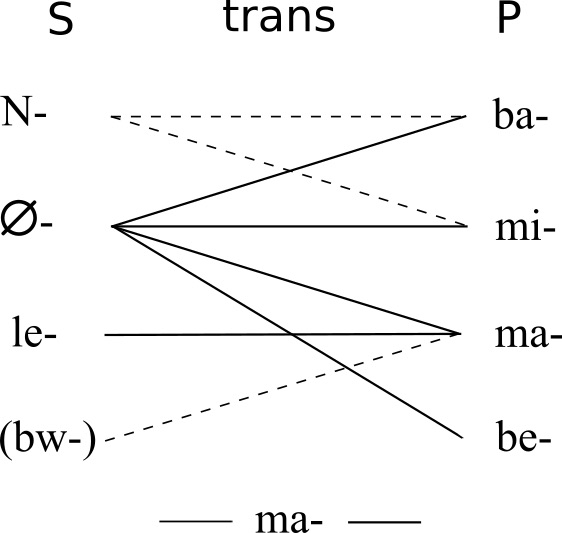
\includegraphics[width=8cm]{figures/Gyeli-NC-system.jpg}
\caption{Noun class pairings}
\label{Fig:NCs}
\end{figure}

\noindent Though the number of major noun class pairings, including the transnumeral category, and the number of major genders is equal, the patterns in which noun classes and agreement classes pair are substantially different. (For comparison, see \sectref{sec:genders}.)\footnote{For both noun and agreement classes, the decision on what constitutes a major versus a minor class is based on frequency. I consider all classes as major if they are represented by 4\% or more in the noun database.}

Table \ref{Tab:NCpair} shows the frequency of each noun class pairing. Just as noun classes by themselves, also their pairings differ significantly in size. For instance, while the smaller noun class pairings such as $\emptyset$/ma- or the transnumeral noun class `ma'- each cover only a little more than 4\%  of the noun database, the largest noun class pairing, $\emptyset$/be-, constitutes a third of all noun class pairings. 
In addition to the 37 nouns in the transnumeral `ma'- class, there are another 35 nouns that lack a singular or plural form. These are subsumed under ``minor transnumerals''. Their distribution is further specified in Table \ref{Tab:genderno}.


\begin{table} 
\centering
\begin{tabular}{l|ll}
 \midrule
Noun class pairing	&  \multicolumn{2}{l}{Frequency} \\  \midrule
N-/ba 			& 23 & (2.6\%) \\
N-/mi- 			&   3 &  (.3\%) \\
$\emptyset$/ba- 	& 139  & (15.9\%) \\
$\emptyset$/mi- 	&   165 & (18.9\%) \\
$\emptyset$/ma- 	&   40  &  (4.6\%) \\
$\emptyset$/be- 	&   296 &  (33.8\%) \\
le-/ma- 			&   136 &  (15.6\%) \\
(bw-/ma-) 		&    1    &  (.1\%) \\
ma- 				&  37   &  (4.2\%) \\
(Minor transnumerals) & 35  & (4\%) \\  \midrule
Total 			& 875 & \\  \midrule
\end{tabular}
\caption{Frequency of noun class pairings}
\label{Tab:NCpair}
\end{table}





\subsection{The Gyeli gender system}
\label{sec:genders}

The nine agreement classes in Gyeli form six major genders, as illustrated in Figure \ref{Fig:Gender}. The major genders are pairings of agreement classes 1/2, 3/4, 5/6, 7/8, and 9/6. Further, the language has a transnumeral gender which does not involve a singular-plural pairing. Instead, nouns only appear in agreement class 6.
There are other nouns which do not have a counterpart in the singular or plural either, but which occur in only one number category.  This ties in with mass and/or abstract nouns and countability and is discussed in \sectref{sec:mass}.

\begin{figure} 
\centering
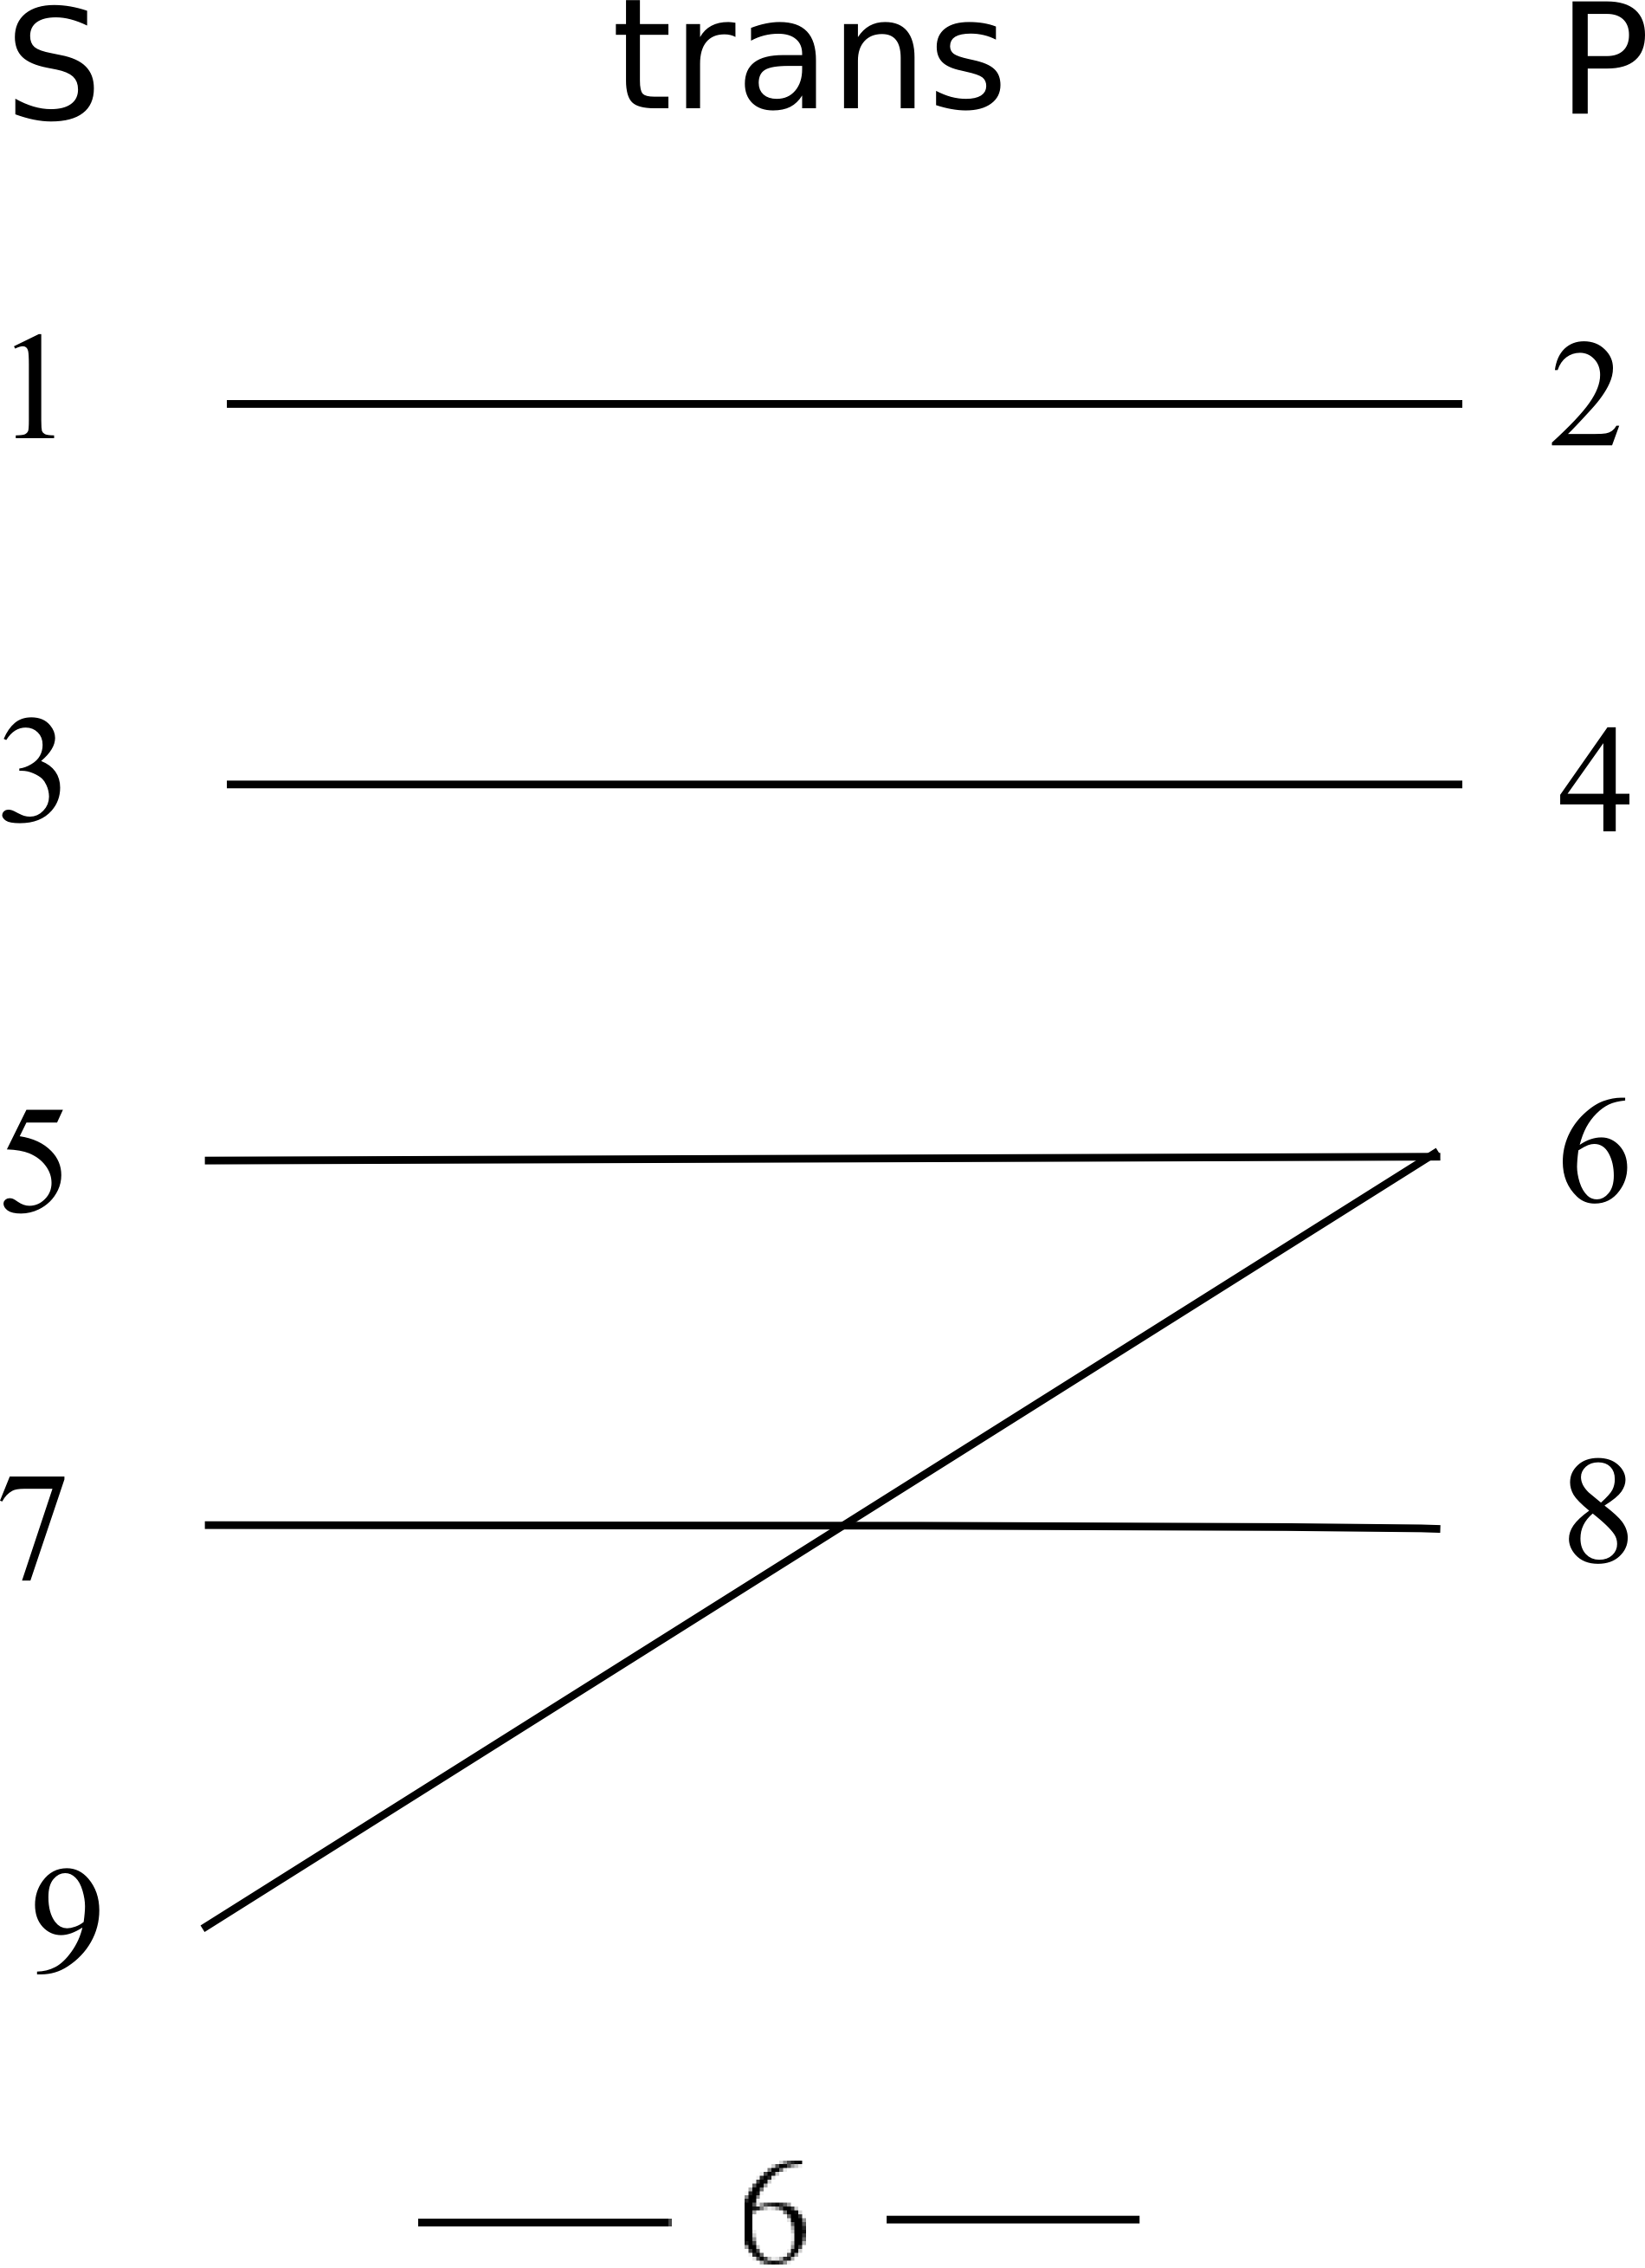
\includegraphics[width=8cm]{figures/Gyeli-gender-system.png}
\caption{Major genders in Gyeli}
\label{Fig:Gender}
\end{figure}

 There are other minor pairings of agreement classes which I do not consider as major, but inquorate genders since they have a limited number of members. They include, for instance, the inquorate genders 7/6, 3/6, 7/0, and 0/8 which I discuss below in gender size.


\paragraph{Gender assignment} \citet{wals-32} states that the way nouns are assigned to a gender can be either strictly semantic, predominantly semantic, or be based on a combination of semantic and formal criteria. In strictly semantic systems, the affiliation of a noun to a gender can be deduced from its meaning. Predominantly semantic systems have more complex assignment rules and therefore the semantic grounds on which affiliation to a gender is based appears less clearly. \citet[2]{wals-32} notes that in these languages, ``for at least some nouns there is no longer a principle for assignment which is still ``live'' for current speakers.'' %He states, however, that nouns that cannot obviously be affiliated to a gender according to their meaning be a minority of exceptions. 
Finally, formal criteria both phonological and morphological can in some languages account for assignment of a noun to a gender, but there are no gender assignment systems that are entirely form based, they rather occur in a combination with semantic assignment criteria (Corbett 2013: 3).


For Bantu languages, \citet[map 32]{wals-32} states in the WALS that gender is typically assigned on both semantic and morphological grounds.
In Gyeli, semantic affiliation of a noun to a certain gender is often opaque and semantic principles governing gender assignment are much less clear-cut, at least synchronically. One cannot say, for instance, that nouns designating humans belong to gender 1/2 which is the typical `human' gender in Bantu languages. It is true that a large part of gender 1/2 comprises humans, but words for humans are also found in almost all the other genders. The same is true for animals, body parts, tools, plants, and other semantic fields. Not one of them is exclusively found in one gender, but spread across several genders.\footnote{\citet[3]{contini2000}  claims in her cognitive grammar approach on Swahili that ``[n]oun classes [are] semantic in origin but [...] have lost much of their semantic coherence over time.'' In order to verify whether this claim applies to Gyeli as well, much more data would be required which exceeds the limits of this grammar.}

It is rather a question of frequency which makes for the typicality of a noun belonging to a certain semantic field to be assigned to a specific gender. Thus, even though human nouns are found in many genders, they are most frequently and thus most typically found in gender 1/2.  
Another tendency in gender assignment concerns loan words which are most frequently found in gender 1/2 and less often in gender 7/8.
 Other patterns, if there are any, are less obvious.

\paragraph{Gender size} The various genders differ in size, i.e.\ the number of members they have. 
Table \ref{Tab:genderno} shows the distribution of the 875 lexemes in the nominal database across different genders, distinguishing major and inquorate genders.\footnote{I consider all genders as major which have a representation of more than 4\% in the database. All other genders, both agreement class pairings and transnumeral genders, are inquorate genders.}


\begin{table} 
\centering
\begin{tabular}{p{4cm}l|ll}
 \midrule
 & Gender &  \multicolumn{2}{l}{Frequency}  \\ 
 \midrule
 \multirow{6}{*}{{\bfseries Major genders}} & 1/2 & 162 & (18.5\%)  \\ 
 & 3/4  & 165 & (18.9\%) \\
 & 5/6  & 136 & (15.5\%)   \\ 
& 7/8   & 270 & (30.9\%) \\
& 9/6   & 40  & (4.6\%) \\ 
 & 6 &  37 &  (4.3\%) \\ 
 \midrule % minor genders
 \multirow{11}{*}{{\bfseries Inquorate genders}} &  7/6  & 24  & (2.7\%) \\
 & 7   & 13  & (1.5\%) \\
 & 8   & 12  & (1.4\%) \\
 & 9   & 3  & (.3\%) \\
 & 3/6  & 2  & (.2\%) \\
 & 8/6   &  2 & (.2\%) \\
& 8/8   & 2 & (.2\%) \\
% \midrule         % transnumeral genders
&  4   & 2  & (.2\%) \\
 & 1   & 2  & (.2\%) \\
 & 3   & 2  & (.2\%) \\
 & 5   & 1  & (.1\%) \\
 \midrule
Total & &  875 & \\
 \midrule
\end{tabular}
\caption{Frequency of genders}
\label{Tab:genderno}
\end{table}

The largest gender is gender 7/8 with over 30\% of the nouns in the database, followed by genders 3/4 and 1/2. The major genders with the least members are genders 9/6 and the transnumeral gender 6. The pairing of agreement classes 7 and 6  constitutes the largest inquorate gender, representing 2.7\% lexemes in the noun database. Other inquorate genders with more than 1\% are the transnumeral genders 7 and 8 while all other exceptional patterns are only represented between one and three times in the noun database.

In the following, I discuss each gender in turn, including examples and semantic tendencies relating to the semantic field of a noun. In order to determine the semantic field of a noun, I coded nominal entries according to the database \citet{haspelmath2009} use in their world loanword typology. The authors distinguish 24 categories differenciating, for instance, `the physical world', `kinship', `animals', `body', `food and drink', clothing', `house', `vegetation', `technology', or `time'.\footnote{For a complete list of all categories and their affiliated lexemes as well as their coding, see \citet[22-34]{haspelmath2009}.}

\subsubsection{Gender 1/2} 
\label{sec:1/2}

Gender 1/2  is a fairly large gender with regard to the number of nouns that are assigned to it with 162 members out of 875 nominal lexical entries. This gender is traditionally referred to as the `human' gender in Bantu studies, but seems to have been extended to an `animate' gender in Gyeli.  Only about 30\% of the nouns do refer to humans (if one excludes agentive deverbal nouns). Most of these human nouns designate kinship and a few social relations as shown in (\ref{1/2kin}) and (\ref{1/2soc}). In comparison to other genders containing human nouns, however, gender 1/2 contains the vast majority.

\begin{exe}
\ex\label{1/2kin} kin relations
\begin{xlist}
\ex sã́/ba-sã́ `father'
\ex nyã̂/ba-nyã̂ `mother'
\ex n-túmbà/ba-túmbà `older male relative'
\ex ntɛ̀mbɔ́/ba-ntɛ̀mbɔ́ `younger sibling'
\ex kálɛ́/ba-kálɛ́ `older sister'
\end{xlist}
\end{exe}

\begin{exe}
\ex\label{1/2soc} social relations
\begin{xlist}
\ex sɔ́/ba-sɔ́ `friend'
\ex n-gyɛ̃̂/ba-gyɛ̃̂ `stranger'
\ex kfúmá/ba-kfúmá `chief'
\ex mbúmbù/ba-mbúmbù `person with the same name'
\ex ngã̂ngã̂/ba-ngã̂ngã̂ `healer'
\end{xlist}
\end{exe}

\noindent 39\% of the gender's nouns belong to the semantic field of animals, both bigger and smaller, as illustrated in (\ref{1/2animals}).

\begin{exe}
\ex\label{1/2animals} animals
\begin{xlist}
\ex tsídí/ba-tsídí `animal, meat'
\ex kímì/ba-kímì `monkey'
\ex nyû/ba-nyû `bee'
\ex fû/ba-fû `fish'
\ex nyúà/ba-nyúà `snake'
\end{xlist}
\end{exe}

\noindent  The remaining 30\% cover a variety of semantic fields such as `food', `
clothing', `house', `vegetation', or `modern world'. It is remarkable that at least more than a third of them constitute loan words that are borrowed especially from English and French as shown in (\ref{1/2loan}). They designate most often recently introduced items in the area of clothing, food, and the modern world.

\begin{exe}
\ex\label{1/2loan} loan words
\begin{xlist}
\ex sɔ́tì/ba-sɔ́tì `trousers (> English: shorts)'
\ex fàrínì/ba-fàrínì `flour (> French: {\itshape farine})'
\ex mɔ̀nɛ́/ba-mɔ̀nɛ́ `money'
\ex màtèlà/ba-màtèlà `mattress'
\ex ngóvìnà/ba-ngóvìnà `government'
\end{xlist}
\end{exe}

\noindent Finally, the absence of a semantic field may be remarkable as well. While `body' nouns\footnote{Note that the semantic field `body' not only contains body parts, but also body functions, health and disease vocabulary as well as terms related to life cycles.} are found with a relatively high percentage in all other genders, they are basically absent in gender 1/2. So far, I only found three instances, all of which designate humans that have a health problem, such as {\itshape njímí/ba-njímí} `blind person', {\itshape búɔ̀/ba-búɔ̀} `mute person', and {\itshape nɔ́ɔ́/ba-nɔ́ɔ́} `deaf person'. Body parts, however, are completely absent in this gender.

\subsubsection{Gender 3/4} 
\label{sec:3/4}

Gender 3/4 is about the same size as gender 1/2 with 165 members out of 875 nominal lexemes. In terms of the meaning of its nouns, the gender is more diverse concerning the semantic fields it covers. The biggest part of its vocabulary belongs to the body parts field with about 27\%, examples of which are given in (\ref{3/4body}).

\begin{exe}
\ex\label{3/4body} body
\begin{xlist}
\ex nlô/mi-nlô `head'
\ex d-ìsì/m-ìsì `eye'
\ex nyùmbù/mi-nyùmbù `mouth'
\ex mɔ̀/mi-mɔ̀ `stomach'
\ex n-sùnɛ̀/mi-sùnɛ̀ `calf'
\end{xlist}
\end{exe}

\noindent Examples in (\ref{3/4world}) represent the next biggest semantic field in gender 3/4 with about 14\% of nouns designating objects in the `physical world'.

\begin{exe}
\ex\label{3/4world} physical world
\begin{xlist}
\ex nsá/mi-nsá `shore'
\ex nkìyɔ́/mi-nkìyɔ́ `wave'
\ex mpá/mi-mpá `island'
\ex nsɛ́/mi-nsɛ́ `sand'
\ex nkúdɛ́/mi-nkúdɛ́ `cloud'
\end{xlist}
\end{exe}

\noindent Further, a relatively large part (11\%) of the lexicon in gender 3/4 designates what the Loanword Database labels as `basic actions/technology', as exemplified in (\ref{3/4tech}). 

\begin{exe}
\ex\label{3/4tech} technology
\begin{xlist}
\ex ntúmɛ́/mi-ntúmɛ́ `walking stick'
\ex ntúmò/mi-ntúmò `knife'
\ex nkwɛ̌/mi-nkwɛ̌ `basket'
\ex nkúnkúmbɛ́/mi-nkúnkúmbɛ́ `bow'
\ex nkwálá/mi-nkwálá `machete'
\end{xlist}
\end{exe}

\noindent Animals are also represented in this gender with more than 8\%; (\ref{3/4animal}) gives examples of some of them.

\begin{exe}
\ex\label{3/4animal} animals
\begin{xlist}
\ex ntsã̂ntsúgɛ́/mi-ntsã̂ntúgɛ́ `dragon fly'
\ex nsĩ̂/mi-nsĩ̂ `mangoost'
\ex nkâ/mi-nkâ `colobus monkey'
\ex nkwúlɔ́/mi-nkwúlɔ́ `cricket'
\ex mbúlɔ̀/mi-mbúlɔ̀ `locust'
\end{xlist}
\end{exe}

\noindent Nevertheless, the remaining 40\% of nouns cover a wide range of semantic fields including `food', `kin', `house', `vegetation', `language', and `time', as illustrated in (\ref{3/4other}), just to mention a few. 

\begin{exe}
\ex\label{3/4other}  others
\begin{xlist}
\ex nkwànɔ̀/mi-nkwànɔ̀ `honey'
\ex mbàmbà/mi-mbàmbà `co-wife'
\ex mbɛ̂/mi-mbɛ̂ `door'
\ex mpìngá/mi-mpìngá `cassava'
\ex nlâ/mi-nlã̂ `story'
\ex mbû/mi-mbvû `year'
\end{xlist}
\end{exe}


\subsubsection{Gender 5/6}
\label{sec:5/6}

Gender 5/6 is slightly smaller than genders 3/4 and 1/2 with 136 members. Like gender 3/4, it contains many body parts (\ref{5/6body}), namely 33\%. The assignment of a body part noun to gender 3/4 or 5/6 seems to be arbitrary since no semantic or form based pattern is obviously descernible.

\begin{exe}
\ex\label{5/6body} body
\begin{xlist}
\ex d-úú/m-úú `nose'
\ex le-lɔ̂/ma-lɔ̂ `ear'
\ex le-nkɛ́dɛ́/ma-nkɛ́dɛ́ `hip'
\ex le-tɔ́lɛ̀/ma-tɔ́lɛ̀ `navel'
\ex le-bɛ́lɛ̀/ma-bɛ́lɛ̀ `breast'
\end{xlist}
\end{exe}

\noindent Further, gender 5/6 contains roughly 19\% animal nouns. Judging from  examples such as in (\ref{5/6animals}), size or habitat of an animal seem not to determine its gender affiliation since quite a range of different animals are found in this gender.

\begin{exe}
\ex\label{5/6animals} animals
\begin{xlist}
\ex le-bóndó/ma-bóndó `frog'
\ex d-á/m-á `crab'
\ex le-bwǐ/ma-bwǐ `hyena'
\ex le-kénó/ma-kénó `duiker'
\ex j-áwɛ̀/m-áwɛ̀ `goliath frog ({\itshape Conraua goliath})'
\end{xlist}
\end{exe}

\noindent Also humans are found in this gender which, according to the Loanword Database, are spread over various semantic fields such as `kin', `social relations', `religion', and `body' (for the `defective' or sick humans). (\ref{5/6hum}). Taking these different categories together, human nouns make up 9\% of gender 5/6.

\begin{exe}
\ex\label{5/6hum} humans
\begin{xlist}
\ex le-wǎ/ma-wǎ `twin'
\ex le-wányɛ̀/ma-wányɛ̀ `young man'
\ex le-kàgà/ma-kàgà `bewitched woman'
\ex le-tɔ́ndí/ma-tɔ́ndí `lover'
\ex le-bùɔ́/ma-bùɔ́ `cripple'
\end{xlist}
\end{exe}

\noindent Further, gender 5/6 includes a small number of nouns belonging to the domain of `house' and the `physical world' with about 7\% each and exemplified in (\ref{5/6house}) and (\ref{5/6world}) respectively.

\begin{exe}
\ex\label{5/6house} house
\begin{xlist}
\ex le-wùdɛ̀/ma-wùdɛ̀ `cooking stone'
\ex d-ù/m-ù `oven'
\ex d-ɛ́ndɛ̀/m-ɛ́ndɛ̀ `courtyard'
\ex d-úgó/m-úgó `toilet'
\ex le-yímbálî/ma-yímbálî `entrance' 
\end{xlist}
\end{exe}

\begin{exe}
\ex\label{5/6world} physical world
\begin{xlist}
\ex le-nángá/ma-nángá `star'
\ex le-bàdà/ma-bàdà `ground'
\ex le-kɔ́/ma-kɔ́ `stone'
\ex le-lɔ̀ɔ́/ma-lɔ̀ɔ́ `dew'
\ex le-tɔ́/ma-tɔ́ `drop'
\end{xlist}
\end{exe}

\noindent The remaining quarter of gender 5/6 nouns is spread across semantic fields such as `vegetation', `technology', `quantity', `time', `language', and `hunting'. (\ref{5/6other}) gives a few examples.

\begin{exe}
\ex\label{5/6other} other
\begin{xlist}
\ex le-lɛ́ndɛ́/ma-lɛ́ndɛ́ `palm tree'
\ex le-kúndí/ma-kúndí `mat'
\ex le-wúmɔ̀/ma-wúmɔ̀ `ten'
\ex le-wùlá/ma-wùlá `hour, time'
\ex le-kɛ́lɛ́/ma-kɛ́lɛ́ `language'
\ex le-lámbɔ̀/ma-lámbɔ̀ `trap'
\end{xlist}
\end{exe}

\noindent Finally, gender 5/6 contains a number of deverbal nouns which are discussed in \sectref{sec:NOM}.


\subsubsection{Gender 7/8}
\label{sec:7/8}

Gender 7/8a is the largest gender in terms of its affiliated nouns with 270 members. `Body' (\ref{7/8body}) and `animal' (\ref{7/8animals}) nouns constitute the majority with both around 20\%. 

\begin{exe}
\ex\label{7/8body} body
\begin{xlist}
\ex vìnɔ́/be-vìnɔ́ `finger'
\ex dò/be-dò `thigh'
\ex sɛ́/be-sɛ́ `liver'
\ex kúdɛ́/be-kúdɛ́ `skin'
\ex gímù/be-gímù `tonge'
\end{xlist}
\end{exe}

\begin{exe}
\ex\label{7/8animals} animals
\begin{xlist}
\ex nɔ̀nɛ́/be-nɔ̀nɛ́ `bird'
\ex tàwɔ̀/be-tàwɔ̀ `goat'
\ex mgbɛ̀mgbɛ̀mɛ̀/be-mgbɛ̀mgbɛ̀mɛ̀ `lion'
\ex sɛ́'ɛ̀/be-sɛ́'ɛ̀ `baboon'
\ex síngì/be-síngì `cat'
\end{xlist}
\end{exe}

\noindent Around 10\% each is taken up by clothing vocabulary as in (\ref{7/8cloth}) and `food' terms as exemplified in (\ref{7/8food}).

\begin{exe}
\ex\label{7/8cloth} clothes
\begin{xlist}
\ex zíngɔ́/be-zíngɔ́ `short dress'
\ex túnɛ̀/be-túnɛ̀ `scarf for carrying babies'
\ex kàbà/b̀e-kàbà `long dress'
\ex tsílì/be-tsílì `long skirt'
\ex póòlì/be-póòlì `hat'
\end{xlist}
\end{exe}

\begin{exe}
\ex\label{7/8food} food
\begin{xlist}
\ex kálá/be-kálá `spice'
\ex kwàndɔ̀/be-kwàndɔ̀ `plantain'
\ex dísì/be-dísì `bowl'
\ex ngùɔ́/be-ngùɔ́ `sugar cane'
\ex búɔ̀/be-búɔ̀ `mortar'
\end{xlist}
\end{exe}

\noindent Another semantic field that is represented in gender 7/8 is `vegetation' as in (\ref{7/8vege}), however, only with around 6\%.

\begin{exe}
\ex\label{7/8vege} vegetation
\begin{xlist}
\ex mpànyè/be-mpànyè `bamboo'
\ex lé/be-lé `tree'
\ex làwɔ́/be-làwɔ́ `branch'
\ex dùwá/be-dùwá `thorn'
\ex kókó/be-kókó `mushroom'
\end{xlist}
\end{exe}

\noindent As in other genders as well, there is a proportion of nouns that belongs to a wide diversity of semantic fields. In gender 7/8, around a third of its member nouns constitute such a semantic diversity. Nouns of semantic fields that are represented with less than 5\% cover semantic domains such as (in decreasing frequency) `language', `physical word', `technology', `house', `hunting', `time', `social/political relations', `spatial relations', and more. An example of each is provided in (\ref{7/8other}).

\begin{exe}
\ex\label{7/8other} other
\begin{xlist}
\ex bã̂/be-bã̂ `word'
\ex nkúdɛ́/be-nkúdɛ́ `fog'
\ex tṹũ̀/be-tṹũ̀ `axe'
\ex pìmáá/be-pìmáá `wall'
\ex bwímɔ̀/be-bwímɔ̀ `net hunt'
\ex mɛ́nɔ́/be-mɛ́nɔ́ `day'
\ex túmbɔ́/be-túmbɔ́ `country'
\ex dyá/be-dyá `distance'
\end{xlist}
\end{exe}

\noindent Finally, gender 7/8 also has a few loan words. This is remarkable because usually loan words are found in gender 1/2. Gender 7/8 seems to be the only other gender that also takes a few borrowed nouns as listed in (\ref{7/8loan}). Compared to gender 1/2, loan words are, however, much less numerous in gender 7/8. 

\begin{exe}
\ex\label{7/8loan} loan words
\begin{xlist}
\ex sɔ́bì/be-sɔ́bì `soap'
\ex fùláwà/be-fùláwà `flower'
\ex súbì/be-súbì `soup'
\end{xlist}
\end{exe}

\noindent It is not clear at this moment, on which grounds loan words get assigned to either one of the two genders that take loan words. If one considers gender 1/2 as the default gender for loan words, it is not clear on which grounds some exceptions are made by assigning loan words to gender 7/8. There is no obvious semantic nor phonological or morphological assignment rule. For instance, {\itshape sɔ́bì} `soap' (gender 7/8) forms a minimal pair with the loan words {\itshape sɔ́tì} `trousers' of gender 1/2. Both nouns belong, according to \citet{haspelmath2009}, semantically to the field of `clothing and grooming'. Another example concerns trisyllabic nouns which start both with /f/ and have the same tonal pattern L H L: {\itshape fùláwà} `flower' belongs to gender 7/8 while {\itshape fàrínì} `flour' belongs to gender 1/2. Gender 7/8 has about 10\% food vocabulary, so it cannot be the case that {\itshape fàrínì} `flour' is not assigned to this gender because it would not fit in semantically. In return, gender 1/2 has some (although few) nouns designating `vegetation', so again it cannot be on semantic grounds that {\itshape fùláwà} `flower' is not assigned to the default loan word gender 1/2. One determining factor could be the donor language . It seems that all loan words in gender 7/8 have an English origin. So far I have not come across any French loan words in this gender. In contrast, loan words in gender 1/2 may come from both English and French. The question still remains then why some English loan nouns are assigned to gender 7/8 while the majority goes into gender 1/2.

\subsubsection{Gender 9/6}
\label{sec:9/6}

Gender 9/6 is the smallest of the major genders with only 40 members in the database of  875 nominal lexemes. Historically, Gyeli has lost agreement class 10 with which agreement class 9 would pair in most other Bantu languages. Instead, Gyeli class 9 pairs synchronically with class 6. In comparison to inquorate genders as discussed in \sectref{sec:MinGen}, gender 9/6 has, however, still more members ($> 4\%$) than the inquorate ones. Even more importantly, agreement class 9 always pairs with agreement class 6 while agreement classes that occur in inquorate genders usually pair with other classes than they do in major genders. 

Semantically, a large part of gender 9/6 nouns (about 29\%) belong to the field of  `body' nouns. Examples are given in (\ref{9/6body}).


\begin{exe}
\ex\label{9/6body} body
\begin{xlist}
\ex nyúlɛ̂/ma-nyúlɛ̂ `body'
\ex mbɔ̀mbɔ́/ma-mbɔ̀mbɔ́ `face'
\ex mbvṹɔ̃̀/ma-mbvṹɔ̃̀ `hair'
\ex tsĩ́/ma-tsĩ́ `neck'
\ex ndzílíkɔ̃̂/ma-ndzílíkɔ̃̂ `elbow'
\end{xlist}
\end{exe}

\noindent Further, a relatively big part (14\%) of gender 9/6 nouns belongs to the semantic field of `language and speech' as illustrated in (\ref{9/6lang}).

\begin{exe}
\ex\label{9/6lang} language
\begin{xlist}
\ex ngɔ̀mɔ̀/ma-ngɔ̀mɔ̀ `little drum (tam tam)'
\ex pɔ́/ma-pɔ́ `news'
\ex tsĩ̂/ma-tsĩ̂ `voice'
\ex mpàálé/ma-mpàálé `message'
\end{xlist}
\end{exe}

\noindent Both, the physical world and `house' vocabulary is represented with about 9\% each and exemplified in (\ref{9/6world}) and (\ref{9/6house}) respectively.

\begin{exe}
\ex\label{9/6world} physical world
\begin{xlist}
\ex mbí'ìlì/ma-mbí'ìlì `charcoal'
\ex sí/ma-sí `ground'
\ex pfùdí/ma-pfùdí `mold'
\end{xlist}
\end{exe}

\begin{exe}
\ex\label{9/6house} house
\begin{xlist}
\ex ndáwɔ̀/ma-ndáwɔ̀ `house'
\ex ntábò/ma-ntábò `washing place'
\ex ngɛ̃̂/ma-ngɛ̃̂ `garden'
\end{xlist}
\end{exe}

\noindent The remaining 40\% of nouns belong to semantic fields such as `food', `technology', `motion', `spatial relations', `law', `religion', and more. Some examples representing the listed semantic domains are given in (\ref{9/6other}).

\begin{exe}
\ex\label{9/6other} others
\begin{xlist}
\ex ndzà/ma-ndzà `hunger'
\ex nkábɛ́/ma-nkábɛ́ `paddle'
\ex ndzì/ma-ndzì `path'
\ex nkwàló/ma-nkwàló `edge'
\ex mpìndá/ma-mpìndá `prohibition'
\ex nkwɛ́lɛ̀/ma-nkwɛ́lɛ̀ `witchcraft'
\end{xlist}
\end{exe}

\subsubsection{Gender 6} 
\label{sec:6}

The transnumeral gender 6 is the smallest of the major genders with only 37 members (4.3\% of nouns in the database). Semantically, it mostly includes liquid mass nouns, as exemplified in (\ref{0/6a}).

\begin{exe}
\ex\label{0/6a}
\begin{xlist}
\ex ma-jíwɔ́ `water'
\ex ma-wã̂ `fat'
\ex ma-nyɔ́ɔ̀ `drink, wine'
\ex ma-nyálɛ̀ `urine'
\ex ma-dyúmù `sperm'
\end{xlist}
\end{exe}

\noindent Other instances of nouns in this gender cover deverbal eventive nouns, as shown in (\ref{0/6b}).

\begin{exe}
\ex\label{0/6b}
\begin{xlist}
\ex ma-dìlá `funeral' $\rightarrow$ dìlɛ `bury'
\ex ma-dígà `vision' $\rightarrow$ dígɛ `watch'
\ex ma-bwálɛ́ `birth' $\rightarrow$ bwálɛ `be born'
\end{xlist}
\end{exe}


\subsection{Inquorate genders}
\label{sec:MinGen}

Inquorate genders are those which have so few members (i.e.\ less than 4\% of the nominal lexemes in the database) that I prefer to treat them as exceptions rather than full-fledged genders in order not to artificially inflate the gender system. Inquorate genders in Gyeli contain the same  agreement classes as major genders. Just their pairing is exceptional. For instance, agreement class 7 usually pairs with agreement class 8. In some exceptions, however, agreement class 7 pairs with class 6 and thus does not belong to the same gender as gender 7/8. Instead, it will be called gender 7/6. Inquorate genders in Gyeli are listed in Table \ref{Tab:genderno}  and will be discussed in order of decreasing member numbers. 

\paragraph{Gender 7/6}

The inquorate gender 7/6 has 24 members in the nominal database. It covers widely diverse semantic fields such as `body', `vegetation', `social relations', `animals', `hunting', or `possession'. (\ref{7/6}) provides some examples.


\begin{exe}
\ex\label{7/6}
\begin{xlist}
\ex bɛ̀/ma-bɛ̀ `shoulder'
\ex ntúà/ma-ntúà `mango'
\ex kwádɔ́/ma-kwádɔ́ `village'
\ex yílì/ma-yílì `viper'
\ex wáádɔ́/ma-wáádɔ́ `net (for hunting)'
\ex mbúlá/ma-mbúlá `debt'
\end{xlist}
\end{exe}

\noindent It is likely that nouns in this minor gender stem from various classes, but it is difficult to trace back since a reconstruction to Proto Bantu (PB) is hardly discernible. Only  {\itshape bɛ̀} `shoulder', out of all 7/6 nouns, can be reconstructed as *-{\itshape bègà} according to \citet[154]{guthrie67}, and belonged to gender 5/6 (Meeussen 1967: 101).%\footnote{There is a tendency in Gyeli to reduce intervocalic word medial (velar) plosives to glottal stops which, in a second step get deleted altogether; the final vowel either gets assimilated to the first or is deleted eventually as well. Thus, some historically bisyllabic nouns in Gyeli tend to be reduced to one syllable.} 
Other nouns such as `debt' or `mango' do not occur in Meeussen's and Guthrie's reconstructions while  {\itshape kwádɔ́} `village' in Gyeli does not seem to have any relation with the PB reconstructions as seen in \citet[27]{guthrie71}. Likewise, it is then not clear whether the singular class of a noun has switched agreement classes or the plural class or whether both scenarios hold for different nouns. 

\paragraph{Gender 7}
The transnumeral gender which only contains the singular agreement class 7 is represented with 13 members in the noun database. It contains a few abstract nouns which lack a plural, as illustrated in (\ref{7/0a}).

\begin{exe}
\ex\label{7/0a}
\begin{xlist}
\ex sɔ́nì `shame'
\ex mɛ̀vâ `pride'
\ex sɔ̀mɔ̀nɛ̀ `complaint'
\ex ngɔ̀ngɔ̀lɛ̀ `sadness'
\ex pɔ́nɛ́ `truth'
\ex ngwámɛ́ `danger'
\end{xlist}
\end{exe}

\noindent Other nouns that only have a singular form in agreement class 7 are country names, as shown in (\ref{7/0b}). 

\begin{exe}
\ex\label{7/0b}
\begin{xlist}
\ex fàlà `France'
\ex ngyàmànɛ̀ `Germany'
\ex ìtálíyɛ̀n `Italy'
\end{xlist}
\end{exe}



\paragraph{Gender 8}
There are also 12 nouns in the database which only have a form in agreement class 8, but no singular or plural counterpart. Like with the transnumeral gender 7, they include abstract nouns, as listed in (\ref{0/8a}). 


\begin{exe}
\ex\label{0/8a}
\begin{xlist}
\ex be-bɛ̃̂ɛ̃̀ `beauty'
\ex be-síyá `imitation'
\ex be-jíì `anger'
\ex be-kílì  `attention, cunning'
\end{xlist}
\end{exe}

\noindent Other nouns of this gender are inherently singular (e.g.\ as a mass noun or a singular occurrence in the world) and lack a plural form, as it is the case with the examples in (\ref{0/8b}).

\begin{exe}
\ex\label{0/8b}
\begin{xlist}
\ex vìyɔ́ `fire'
\ex vísɔ́ `sun'
\end{xlist}
\end{exe}



\paragraph{Gender 9}
Also agreement class 9 constitutes a transnumeral gender with three members. They are listed in (\ref{0/9}).


\begin{exe}
\ex\label{0/9}
\begin{xlist}
\ex ngwɛ́lɛ̀ `witchcraft'
\ex mpà'à `vapor, fog'
\ex bvúbvù `multitude'
\end{xlist}
\end{exe}

\paragraph{Gender 3/6}
Many exceptional agreement class pairings only occur a couple of times in the database. This is the case with the pairing of agreement classes 3 and 6. The only two examples that I found are shown in (\ref{3/6}).


\begin{exe}
\ex\label{3/6}
\begin{xlist}
\ex m-bɔ́/mà-bɔ́ `arm'
\ex n-ákɔ́/m-ákɔ́ `earwax'
\end{xlist}
\end{exe}


\noindent This lexeme -{\itshape bɔ́} `arm' may be reconstructed to PB *{\itshape -bóko} `arm' which belonged to gender 15/6 according to \citet[102]{meeussen67}.\footnote{Other nouns that \citet[102]{meeussen67} classifies as gender 15/6 nouns such as `leg', `knee',  or `ear' do not have any reflexes in synchronic Gyeli. Since many of them constitute body parts, this is, however, not surprising at all. \citet{wilkins96}, for instance, shows that especially body parts, or `parts of a person' terminology, as he labels it, are subject to a great deal of semantic change which follows cross-linguistically natural tendencies. Therefore, synchronic noun stems of body parts may have an entirely different shape than the reconstructed PB forms. In any case, it is not possible to say that historic class 15 nouns merged systematically with class 3.}


\paragraph{Gender 8/6}

Agreement class 8 has a few singular nouns. While the plural nouns of agreement class 8 all belong to noun prefix class `be', the singular members of agreement class 8 do not take a prefix.\footnote{There is one exception where a singular agreement class 8 noun takes a prefix of the shape {\itshape bw}-, a remnant of a former class 14. Since this is the only example, however, I do not list `bw' as a noun prefix class on its own.}
 Historically, agreement class 8 nouns which do not take a prefix have probably merged from a former class 14 as the root  beginning bw- or b- suggests. This would also be in line in with the plural pairing with class 6 since \citet[100]{meeussen67} points out that class 14 in PB formed its plural with class 6. Pairings of class 8/6 are very rare in Gyeli. I only found two examples which are given in (\ref{8/6}).

\begin{exe}
\ex\label{8/6}
\begin{xlist}
\ex bwã̂/ma-bwã̂ `medicine'
\ex bw-álɛ̀/m-álɛ̀ `canoe'
\end{xlist}
\end{exe}



\paragraph{Gender 8/8}
There are two other examples where the singular variant of agreement class 8 pairs with the plural class 8, as shown in (\ref{8/8}). 

\begin{exe}
\ex\label{8/8}
\begin{xlist}
\ex bvùlɛ́/be-bvùlɛ́ `night'
\ex bírɛ̀lɛ̀/be-bírɛ̀lɛ̀ `smoke'
\end{xlist}
\end{exe}

\paragraph{Other exceptional transnumeral genders}

Except for agreement class 2, all agreement classes show instances where they lack either a singular of plural counterpart. For classes 1, 3, 4, and 5, this is very rare with only one or two examples each. (\ref{0/4}) shows the two examples found for agreement class 4.


\begin{exe}
\ex\label{0/4}
\begin{xlist}
\ex mi-ngyɛ̌ `hunting rats (digging out their dens)'
\ex my-ɛ́ `fur'
\end{xlist}
\end{exe}

\noindent Instances where agreement class 1 does not have a plural form concern proper names of countries/continents which are inherently singular, as shown in (\ref{1/0}).

\begin{exe}
\ex\label{1/0}
\begin{xlist}
\ex kàmɛ̀rún `Cameroon'
\ex àfríkà `Africa'
\end{xlist}
\end{exe}

\noindent There are also two examples of agreement class 3 nouns which do not take a plural form in class 4. These are listed in (\ref{3/0}).

\begin{exe}
\ex\label{3/0}
\begin{xlist}
\ex bíwɔ̀ `bad luck'
\ex mbvú `white/grey hair'
\end{xlist}
\end{exe}

\noindent Agreement class 5 only has one instance which lacks a plural counterpart, as shown in (\ref{5/0}).

\begin{exe}
\ex\label{5/0}
 dyúwɔ̀ `sky'
\end{exe}






\subsection{Agreement targets of the noun}
\label{sec:AGRtargets}

The head noun triggers agreement on its agreement targets. While each of the agreement targets is described in detail according to their part of speech in \chapref{sec:POS}, I give an overview of all agreement targets in Table \ref{Tab:AGRtargets}.

\todo[1082]{indent instead of hspace}
\begin{table}[!h]
\begin{tabular}{l|l}
 \midrule
\multirow{ 7}{*}{Noun phrase internal} &   \\
& Modifiers with agreement prefix \\
& \hspace{.5cm}	-{\itshape vúdũ̂} `one' \\
& \hspace{.5cm}	-{\itshape fúsì} `different' \\
& \hspace{.5cm}	-{\itshape ɛ́sɛ̀} `all' \\
& \hspace{.5cm}	-{\itshape ɔ́(nɛ́)gá} `other' \\
& \hspace{.5cm}	numerals `2' through `5' \\
& \hspace{.5cm}	genitive marker {\itshape ngá} \\
& \hspace{.5cm}	{\itshape nyá} `big' \\
& Modifiers with agreeing free morpheme \\
& \hspace{.5cm}	Demonstratives \\
& \hspace{.5cm}	Attributive markers \\  \midrule
\multirow{ 2}{*}{Noun phrase external} & \\
& \hspace{.5cm}	STAMP marker \\
& \hspace{.5cm}	Copula \\
 \midrule
\end{tabular}
\caption{Agreement targets}
\label{Tab:AGRtargets}
\end{table}













 



\section{Distributive numerals with reduplication} 
\label{sec:Distr}
\sectionmark{Distributive numerals}

Distributives form series of numerals which are expressed by repetition of the numeral. They serve the purpose of disambiguating sentences such as in (\ref{Distr}) which can have either a collective or a distributive reading.

\begin{exe}
\ex\label{Distr}
 Finn and Riley ate two apples.
\end{exe}

\noindent In the collective reading, two apples altogether were shared between Finn and Riley whereas in a distributive interpretation, Finn ate two apples and Riley ate two apples. In English, such sentences can be disambiguated by the use of `each': `Finn and Riley ate two apples each.' Sentences as in (\ref{Distr}) are, however, ambiguous and allow for both interpretations.

Some languages have means to regularly disambiguate such cases. For those languages that do that, the most common means is reduplication of numerals. \citet[4]{gil05} explains this common strategy by its iconic motivation. According to him, copies of the numeral correspond to multiple sets of entities.

Gyeli also uses the reduplication strategy in order to express distributive numerals. Even though reduplication is a common strategy for distributive expression in the languages of the world, \citet[3]{rubino05} states that, `The phonological nature of the reduplicated material varies from language to language and construction to construction.''  \citet[118]{borchardt11} shows that the Benue-Congo language Ikaan, for instance, uses several types of reduplication in order to express distributives. These range from full reduplications including the agreement markers to full root reduplications excluding agreement markers and partial root reduplications where only part of the numeral root is copied. 

In Gyeli, distributive numerals only display one kind of reduplication, namely full reduplication. The numeral, based on its cardinal form, is entirely copied, including its agreement prefixes, if required, and tones. (\ref{nut}) illustrates how distributives may be used in Gyeli.

\begin{exe}
\ex\label{nut}
  \glll   bwánɔ̀ bà dé mímbàngá {\bfseries mímbáà} {\bfseries mímbáà}\\
         b-wánɔ̀ ba dè-H mí-mbàngá mí-mbáà mí-mbáà\\
                ba2-child 2.PST1 eat-R mi4-nut 4-two 4-two \\
    \trans `The children ate two nuts each.'
\end{exe}

\noindent Just like cardinals, distributive numerals agree with the head noun in its noun class, if the specific numeral takes an agreement marker. The distributives that take agreement markers are exactly the same as the cardinals that do, namely `2' through `5'. For those modifier numerals that do not take any agreement prefixes (`6' through `9'), they are entirely reduplicated, just without prefixes. Nominal nouns as well as complex numerals involving noun phrases and/or coordination are also fully reduplicated as one would expect from their cardinal form. Table \ref{tab:Distributives} lists Gyeli distributives using the noun {\itshape mbàngá} `nut' of gender 3/4 as an example. 

\begin{table} 
\centering
\begin{tabular}{ll|l}
 \midrule
\multicolumn{2}{c}{Examples of distributive numerals}  & Gloss \\
  \midrule
{\itshape mbàngá} & {\itshape mvúdũ̂ mvúdũ̂} & `one nut each' \\
{\itshape mi-mbàngá} & {\itshape mí-mbáà mí-mbáà} & `two nuts each'\\
{\itshape mi-mbàngá} & {\itshape mí-nláálɛ̀ mí-nláálɛ̀} & `three nuts each' \\
{\itshape mi-mbàngá} & {\itshape mí-nã̂ mí-nã̂} & `four nuts each' \\
{\itshape mi-mbàngá} & {\itshape mí-ntánɛ̀ mí-ntánɛ̀} & `five nuts each' \\
{\itshape mi-mbàngá} & {\itshape ntùɔ́ ntùɔ́} & `six nuts each' \\
{\itshape mi-mbàngá} & {\itshape mpúɛ̀rɛ́ mpúɛ̀rɛ́} & `seven nuts each' \\
{\itshape mi-mbàngá} & {\itshape lɔ̀mbì lɔ̀mbì} & `eight nuts each' \\
{\itshape mi-mbàngá} & {\itshape rèbvùá rèbvùá} & `nine nuts each' \\
{\itshape mi-mbàngá} & {\itshape le-wúmɔ̀ le-wúmɔ̀} & `ten nuts each' \\
{\itshape mi-mbàngá} & {\itshape le-wúmɔ̀ ná mí-báà le-wúmɔ̀ ná mí-báà} & `twelve nuts each' \\
{\itshape mi-mbàngá} & {\itshape ma-wúmɔ̀ má-báà ma-wúmɔ̀ má-báà} & `twenty nuts each' \\
{\itshape mi-mbàngá} & {\itshape bwúyà bwúyà} & `a hundred nuts each' \\
{\itshape mi-mbàngá} & {\itshape tɔ́dyínì tɔ́dyínì} & `a thousand nuts each' \\
  \midrule
\end{tabular}
\caption{Distributive numerals}
\label{tab:Distributives}
\end{table}



\section{Distributive construction with {\itshape náà}} 
\label{sec:RedQUANT}

%[Is reduplication the right term here since there is the {\itshape nâ} in between the two nouns?] [???]


In order to express distributivity over individuals, a (countable) noun is iterated while {\itshape náà} is inserted to link the two nouns. %The status of {\itshape náà} is not entirely clear. It does not seem to be a comitative marker judging from the tones since they come with a L tone. {\itshape náà} rather resembles the adverb {\itshape nâ} `still, again', which, however, has a short vowel instead of a long one. 
The quantified noun can occur both in the singular or in the plural as shown in (\ref{each}). The use of plural nouns as in (\ref{each2}) implies a distribution over a set of entities.  

\begin{exe}
\ex\label{each}
\begin{xlist}
\ex\label{each1}
 \gll  m-ùdì  náà m-ùdì \\
          N1-person by N1-person  \\
    \trans `each person'
\ex \label{each2}
  \gll    b-ùdì  náà b-ùdì \\
             ba2-person by ba2-person \\
    \trans `each (set of) people'
\end {xlist}
\end {exe}

Iterated quantification in the sense of `each' only works for countable nouns. Thus, neither liquid mass nouns nor granular aggregates in their singular form allow for iterated quantification as shown in (\ref{noeach}). Granular aggregates in their plural form, however, can enter such a construction which then gives the reading of `each set of entities of x' as in (\ref{noeach3}).

\begin{exe}
\ex\label{noeach}
\begin{xlist}
\ex\label{noeach1}
 \gll  *ma-jíwɔ́ náà ma-jíwɔ́ \\
          ma6-water by ma6-water  \\
    \trans `each water'
\ex \label{noeach2}
  \gll    *ndísì náà ndísì \\
              $\emptyset$3.rice by nc3.rice \\
    \trans `each rice'
\ex \label{noeach3}
  \gll    mi-ndísì náà mi-ndísì \\
              mi4-rice by nc4-rice \\
    \trans `each set of packages of rice'
\end {xlist}
\end {exe}




\section{Attributive constructions}
\label{sec:CONC}

In his comparative study on Bantu attributive constructions, \citet{velde2013} defines a `canonical' attributive construction as a dependency relation between two nominal constituents. It is also known as associative or genitive constructions in the Bantu literature. Since in Gyeli these constructions are, however, not confined to genitive contexts, I prefer to call them `attributive constructions'.  So, canonically, an attributive (or associative) marker links a head noun with a dependent noun. \citet[217]{velde2013} illustrates this with an example from Kagulu (Bantu G12, Tanzania), cited from \citet[86]{petzell2008} in (\ref{const}).

\begin{exe}
\ex\label{const} Kagulu (Bantu G12) 
  \gll  m-eji\textsubscript{$R1$} g-a\textsubscript{$REL$} mu-nyu\textsubscript{$R2$}\\
              6-water VI-ATT 3-salt\\
    \trans `salt water'
\end{exe}

\noindent \citet{velde2013} describes the canonical attributive construction as HEAD (R1) - RELATOR (REL) - DEPENDENT (R2), where the relator (attributive marker) links the head noun (R1) to the dependent noun (R2).  He further points out that Bantu languages are homogeneous with respect to the way they express attributive possession structurally. There is a huge variation in terms of, for instance, the shape of the attributive marker with a canonical shape of AGR-{\itshape a} (see \sectref{sec:ATT} for the attributive marker). Also, the dependent constituent which is typically a  noun, can also belong to another part of speech. This is the case for Gyeli. In terms of frequency, the dependent constituent is mostly a noun. It can, however, also belong to the category of adjectives, verbs, or interrogative words. While the part of speech of the dependent constituent may belong to various categories, the head of the construction seems always to be a noun. In the following, I will present the different construction types that occur with a noun + POS. 

\subsection{Noun + noun}
\label{sec:NN}

Noun + noun attributive constructions in Gyeli typically express attributive possession. This core meaning, however, which is extended to other semantic properties of a noun, e.g.~quantification ('a lot of cats') and location ('front of the house'). I will discuss in turn the different domains of attributive constructions, starting with the core meaning of possession.

Before turning to the different attributive constructions in Gyeli, however, I will first explore a general formal issue: the optional omission of the attributive marker. The core of a noun + POS construction seems to be the linking element, the attributive marker, which gives the construction its name. Often, the attributive marker can be omitted, while in some cases, it cannot, but must appear. 


\subsubsection{Optional omission of the attributive marker}
\label{sec:CONOM}

 In Gyeli, the attributive marker can in many cases be omitted optionally (which seems to be the default case) as shown in (\ref{mino}). In some special cases, however, the attributive is obligatorily, as in (\ref{djino}).\footnote{Note that attributive markers in parentheses are optional while those without brackets cannot be omitted, but must obligatorily appear.} 

\begin{exe}
\ex\label{mino} 
  \gll     m-ínɔ̀ (má) bá-sɔ́ \\
              ma6-name 6:ATT  ba2-friend\\
    \trans `the friends' names'
\end{exe}

\begin{exe}
\ex\label{djino} 
  \gll     j-ínɔ̀ lé sɔ́ \\
              le5-name 5:ATT  $\emptyset$1.friend\\
    \trans `the friend's name'
\end{exe}

\noindent This phenomenon cannot be based on free variation, but must be conditioned by some (set of) rules since speakers are consistent in their judgments of optional omission or obligatory presence of the attributive.

The question is then what conditions are at play in the presence or absence of the attributive marker. It seems that multiple factors determine whether the attributive marker has to appear, including i) phonological ones where a dependent noun that comes with a CV- shape noun class prefix favors omission of the attributive and ii) semantic ones concerning the relation between the two nouns. In the following, I will go through a number of possible determining factors and point out in how far they might influence the occurrence of an attributive marker. I will start out with phonological factors, then move on to morphological, and finally to semantic factors.

\paragraph{Phonological factors: tonal patterns}

The H tone of an attributive marker spreads on to a CV- noun class prefix of the dependent noun as shown in (\ref{TON}) and discussed in \sectref{sec:HTSr}. One could assume that if the H tone of the attributive marker spreads to the otherwise L tone prefix of the dependent noun R\textsubscript{2}, the tonal process might mark the dependency relation and an overt attributive marker is not necessary as in (\ref{TON2}), while agreement classes that come with a L tone attributive marker where no H tone spreading occurs determine the obligatory use of the attributive as would seem to be the case in (\ref{TON1}).

\begin{exe}
\ex\label{TON}
\begin{xlist}
\ex\label{TON2}
 \gll     mì-nlô (mí) bá-tídí \\
               mi4-head 4:ATT ba2-animal \\
    \trans `the heads of the animals'
\ex \label{TON1}
  \gll     \ nlô wà tsídí \\
               $\emptyset$3.head 3:ATT $\emptyset$1.animal  \\
    \trans `the head of the animal'
\end {xlist}
\end{exe}

This turns out not to be the case, however. (\ref{pres}) counterexemplifies the tonal hypothesis because in (\ref{pres1}), there is no high tone spreading, but the use of the attributive marker is still optional while in (\ref{pres2}) there is high tone spreading, but the use of the attributive marker is still obligatory.

\begin{exe}
\ex\label{pres}
\begin{xlist}
\ex \label{pres1}
  \gll     m-páà (wà) nlàmbɔ́ \\
               N1-president 1:ATT $\emptyset$3.country  \\
    \trans `president of the country'
\ex\label{pres2}
 \gll     bà-páà bá nlàmbɔ́ \\
               ba2-president 2:ATT $\emptyset$3.country \\
    \trans `presidents of the country'
\end {xlist}
\end{exe}

\paragraph{Phonological factors: syllable length} There is a tendency for  monosyllabic dependent nouns R\textsubscript{2} to require an attributive marker rather than allowing for its omission as in (\ref{PHO}) compared to bisyllabic dependent nouns R\textsubscript{2} in (\ref{pho}). A bit more than half of the elicited attributive constructions with monosyllabic R\textsubscript{2} behave this way.%\footnote{[STATE BASIS OF STATISTICS ???]}


\begin{exe}
\ex\label{PHO}
\begin{xlist}
\ex \label{PHO1}
  \gll     sɔ́ wà n-tí \\
               $\emptyset$1.friend 1:ATT N1-in.law \\
    \trans `the friend of the in-law'
\ex\label{PHO2}
 \gll     bà-sɔ́ bá n-tí \\
               ba2-friend 2:ATT N1-in.law \\
    \trans `the friends of the in-law'
\end {xlist}
\end{exe}


\begin{exe}
\ex\label{pho}
\begin{xlist}
\ex \label{pho1}
  \gll     sɔ́ (wà) bà-tí \\
               $\emptyset$1.friend 1:ATT ba2-in.law  \\
    \trans `the friend of the in-laws'
\ex\label{pho2}
 \gll     bà-sɔ́ (bá) bá-tí  \\
               ba2-friend 2:ATT ba2-in.law \\
    \trans `friends of the in-laws'
\end {xlist}
\end{exe}


\noindent There are, however, many exceptions as in (\ref{syll}) where the dependent noun R\textsubscript{2} is monosyllabic, but the use of the attributive marker is still optional.

\begin{exe}
\ex\label{syll}
\begin{xlist}
\ex \label{syll1}
  \gll     ndzí (nyà) nsɛ́ \\
              $\emptyset$9.path 9:ATT $\emptyset$3.sand   \\
    \trans `path of sand'
\ex\label{syll2}
 \gll   j-ìnɔ́ (lé) n-tí   \\
              le5-name 5:ATT N3-in.law \\
    \trans `the name of the in-law'
\end {xlist}
\end{exe}

\noindent At the same time, these examples concerning syllable length could also relate to number morphology. Monosyllabic nouns are almost exclusively singular while plural nouns are almost exclusively at least bisyllabic. So the question is whether a possibly conditioning factor is about syllable length or rather about number morphology or agreement class affiliation.

\paragraph{Morphological factors: number of R\textsubscript{2}} Another factor that seems to determine the obligatory presence of the attributive marker is the number of the dependent noun R\textsubscript{2}. If R\textsubscript{2} occurs in the singular, the attributive occurrence is often (more than 50\% of the elicited examples) obligatory as exemplified in (\ref{pl1}). In fact, out of all cases where the attributive linker is obligatory, more than 75 \% have a singular dependent noun R\textsubscript{2}. In contrast, if R\textsubscript{2} is plural as in (\ref{pl2}), the use of the attributive is mostly optional. 


\begin{exe}
\ex\label{pl}
\begin{xlist}
\ex \label{pl1}
  \gll     ndzí nyà táwɔ̀ \\
               $\emptyset$9.path 9:ATT $\emptyset$7.goat \\
    \trans `path of the goat'
\ex\label{pl2}
 \gll     ndzí (nyà) bè-táwɔ̀ \\
               $\emptyset$9.path 9:ATT be8-goat \\
    \trans `path of the goats'
\end {xlist}
\end{exe}

\noindent Again, there are examples, such as in (\ref{crab}), where the inverse is the case.

\begin{exe}
\ex\label{crab}
\begin{xlist}
\ex \label{crab1}
  \gll    j-ìnɔ́ (lé) d-á'á \\
               le5-name 5:ATT le5-crab \\
    \trans `name of the crab'
\ex\label{crab2}
 \gll     j-ìnɔ́ lé m-á'á \\
              le5-name 5:ATT ma6-crab \\
    \trans `name of the crabs'
\end {xlist}
\end{exe}

\paragraph{Morphological factors: noun class affiliation} Another hypothesis could be that attributive marker optionality is conditioned by gender or agreement class and depends on the gender/noun class of the head noun R\textsubscript{1} or the dependent noun R\textsubscript{2}. This is in fact the case in many closely related languages as described by \citet{henson2007} for Kol (A832),\footnote{\citet[113]{henson2007}  points out for Kol that "For most singular nouns, the `basic' associative marker is either zero or a tonal marker".} by \citet{beavon2006} for Njyem (A84)\footnote{\citet[118]{beavon2006} shows that head nouns of classes 1, 9, and 10 in Njyem occur without associative markers.} and by \citet{heath2003} for Makaa (A83).\footnote{As in Njyem, head nouns of classes 1, 9, and 10 in Makaa do not come with an associative marker and are therefore zero-marked  in noun + noun constructions according to \citet[341]{heath2003}.} For Gyeli, however, this does not seem to be the case for either the head nor the dependent noun. Changing the noun class of R\textsubscript{1} in (\ref{R1}) gives both optional omission of the attributive as in (\ref{R11}) and obligatory use of the attributive marker as in (\ref{R12}).

\begin{exe}
\ex\label{R1}
\begin{xlist}
\ex \label{R11}
  \gll     sɔ́ (wà) n-gyɛ̃̂ \\
               $\emptyset$1.friend 1:ATT N1-stranger \\
    \trans `friend of the stranger'
\ex\label{R12}
 \gll     ndzí nyà n-gyɛ̃̂ \\
               $\emptyset$9.path 9:ATT N1-stranger \\
    \trans `path of the stranger'
\end {xlist}
\end{exe}


\noindent The same is true for the dependent noun R\textsubscript{2} in (\ref{R2}): (\ref{R21}) shows a case where the attributive can be omitted while it cannot in (\ref{R22}).

\begin{exe}
\ex\label{R2}
\begin{xlist}
\ex \label{R21}
  \gll     sɔ́ (wà) m-ùdã̂ \\
               friend.1 1:ATT  N1-woman \\
    \trans `friend of the woman'
\ex\label{R22}
 \gll     sɔ́ wà nkwànò \\
               $\emptyset$1.friend 1:ATT $\emptyset$3.honey \\
    \trans `friend of honey' (= somebody who likes honey)
\end {xlist}
\end{exe}

\noindent It also does not depend on whether  the head noun R\textsubscript{1} and the dependent noun R\textsubscript{2} belong to the same noun class or not: in (\ref{7}), all constituents belong to noun class 7. In (\ref{71}), the use of the attributive is obligatory while in (\ref{72}) its use is optional.

\begin{exe}
\ex\label{7}
\begin{xlist}
\ex \label{71}
  \gll     vɛ́ɛ̀lá yá yí \\
              $\emptyset$7.decoration 7:ATT $\emptyset$7.wood \\
    \trans `decoration of the wood'
\ex\label{72}
 \gll    vɛ́ɛ̀lá (yá) táwɔ̀  \\
             $\emptyset$7.decoration 7:ATT $\emptyset$7.goat   \\
    \trans `decoration of the goat'
\end {xlist}
\end{exe}

\paragraph{Morphological factors: overt noun class marking of R\textsubscript{2}} There is a  tendency to omit the attributive marker when the dependent noun R\textsubscript{2} has a syllabic noun class prefix as seen for instance in (\ref{TON2}) or (\ref{pho1}). This is true for more than 80\% of the elicited attributive construction examples.

Further, at the intersection of phonology and morphology, there is a tendency to avoid successive identical CV morphemes, i.e.~when the attributive marker and the following noun class prefix have the same CV pattern as in (\ref{double}). In more than 90\% of these cases, speakers prefer to omit the attributive.

\begin{exe}
\ex\label{double}
\begin{xlist}
\ex \label{double1}
  \gll     bà-sɔ́ (bá) bá-tí \\
               ba2-friend 2:ATT ba2-in.law \\
    \trans `the friends of the in-laws'
\ex\label{double2}
 \gll    j-ìnɔ́ (lé) lé-kǎ \\
             le5-name 5:ATT le5-clan   \\
    \trans `the name of the clan'
\end {xlist}
\end{exe}

\noindent Nevertheless, there are again counterexamples as in (\ref{fever}).

\begin{exe}
\ex\label{fever}
  \gll     mà-dyû má má-kǎ \\
               ma6-fever 6:ATT ma6-clan \\
    \trans `the fevers of the clans'
\end{exe}

\paragraph{Semantic factors: relation between the nouns} It seems that the attributive linker can be omitted when the relation between the two nouns is an identity relation as with names in (\ref{name}) and colors in (\ref{color}).

\begin{exe} 
\ex\label{name}
  \gll     kwádɔ́ (yá) Ngòló \\
               $\emptyset$7.village 7:ATT $\emptyset$3.PN \\
    \trans `the village of Ngolo'
\end{exe}

\begin{exe} 
\ex\label{color}
  \gll     nsínó (wá) nábèbè \\
               $\emptyset$3.color 3:ATT red \\
    \trans `the color red'
\end{exe}

\noindent Also numeral head nouns are always followed by an optional attributive marker as shown in (\ref{num}).

\begin{exe}
\ex\label{num}
\begin{xlist}
\ex \label{num1}
  \gll     lè-wúmɔ̀ (lé) bá-sɔ́ \\
               le5-ten 5:ATT ba2-friend  \\
    \trans `ten friends'
\ex\label{num2}
 \gll     bwúyà (yá) bá-sɔ́ \\
              $\emptyset$7.hundred 7:ATT ba2-friend \\
    \trans `hundred friends'
    \ex\label{num3}
 \gll     tɔ́gyínì (wà) bà-sɔ́ \\
              $\emptyset$1.thousand 1:ATT ba2-friend  \\
    \trans `thousand friends'
\end {xlist}
\end{exe}

Further, the omission of the attributive marker changes, in some cases, the meaning of the construction which supports the hypothesis on identity relation: if the head and dependent noun refer to the same entity, the attributive can or even must be omitted as in (\ref{woman2}) and (\ref{chick2}).  In these cases, the second noun rather serves as a modifying noun to the head. In contrast, (\ref{woman1}) and (\ref{chick1}) which require the attributive marker, are attributive possession constructions.

\begin{exe}
\ex\label{woman}
\begin{xlist}
\ex\label{woman2}
 \gll     sɔ́ m-ùdã̂ \\
              $\emptyset$1.friend N1-woman \\
    \trans `the female friend'
\ex \label{woman1}
  \gll    sɔ́ wà m-ùdã̂ \\
               $\emptyset$1.friend 1:ATT N1-woman \\
    \trans `the friend of the woman'
\end {xlist}
\end{exe}

\begin{exe}
\ex\label{chick}
\begin{xlist}
\ex\label{chick2}
 \gll     kfúbɔ̀ dyá \\
            $\emptyset$1.chicken $\emptyset$7.length   \\
    \trans `the tall chicken'
\ex \label{chick1}
  \gll    kfúbɔ̀ wà dyá \\
              $\emptyset$1.chicken 1:ATT $\emptyset$7.length \\
    \trans `the chicken that is far away' (poulet eloigné)
\end {xlist}
\end{exe}

\paragraph{Semantic factors: prototypical use} A final factor that I consider here concerns prototypicality of use which relates to the most frequent, most natural way, two nouns are linked. In (\ref{country}), for instance, it seems that speakers natuarlly think of a country usually having only one president. In this case (\ref{country1}), the attributive can be omitted. If, however, speakers talk about several presidents as in (\ref{country1}), for instance historically successive presidents, this is the more marked form and there the use of the attributive is obligatory.

\begin{exe}
\ex\label{country}
\begin{xlist}
\ex \label{country1}
  \gll     m-páà (wà) nlàmbɔ́ \\
               N1-president 1:ATT $\emptyset$3.country  \\
    \trans `president of the country'
\ex\label{country2}
 \gll     bà-páà bá nlàmbɔ́ \\
               ba2-president 2:ATT $\emptyset$3.country \\
    \trans `presidents of the country'
\end {xlist}
\end{exe}


It has to be noted that there might be other factors at play as well and also that there seem always  to be exceptions to the rules and that these rules are rather tendencies. Ultimately, it is not completely clear at this moment what makes attributive occurrence obligatory, also because it is not clear in which way the different factors interact. 

\subsubsection{Nominal possessives}  
\label{sec:NomPOSS}

Having discussed the optional omission and obligatory presence of the attributive marker in noun + noun constructions, I will for reasons of simplicity in the following not indicate anymore, whether the attributive is optional or not. After having discussed the formal side of noun + noun attributive constructions, I now turn to semantically different noun + noun constructions. The core meaning of these is that of attributive possession. Examples of possessive noun + noun constructions are given in (\ref{possession}), where the head noun changes noun class. The head noun expresses the possessee while the dependent noun expresses the possessor.

\begin{exe}
\ex\label{possession}
\begin{xlist}
\ex \label{possession1}
  \gll     m-ùdã̂ wà m-ùdì \\
               N1-woman 1:ATT N1-person  \\
    \trans `the person's wife'
\ex \label{possession2}
  \gll     b-ùdã̂ bá m-ùdì \\
               ba2-woman 2:ATT N1-person  \\
    \trans `the person's wives'
\ex \label{possession3}
  \gll     d-ìsí lé m-ùdì \\
               le5-eye 5:ATT N1-person  \\
    \trans `the person's eye'
\ex \label{possession4}
  \gll     m-ísì má m-ùdì \\
               ma6-eye 6:ATT N1-person  \\
    \trans `the person's eyes'
\end {xlist}
\end{exe}

\paragraph{Split genitive} Gyeli has a split genitive system. Interestingly, the language has, however, not a typical possessive classification system which most often  distinguishes grammatically between alienable and inalienable possession. \citet{nichols2013} explain that this type of possessive classification is based on properties of the possessee. Typically, inalienable possession concern kinship relations and body parts while alienable possessions can be separated from the owner, for instance materials (axe, spear) or food items (mango, bread). According to the WALS map on possessive classification by \citet{nichols2013}, some Niger-Congo languages such as Gbeya Bossangoa (Central African Republic), Lango and Luganda (Uganda), or Luvale (Angola) have a two possessive classes with an alienable/inalienable distinction.

Gyeli does not make a grammatical distinction between alienable and inalienable possession as shown in (\ref{INAL}). No matter whether the possessee is a kin (\ref{INAL1}), body part (\ref{INAL2}), or material possession (\ref{INAL3}), the attributive marker always agrees in class with the head noun (possessee).

\begin{exe}
\ex\label{INAL}
\begin{xlist}
\ex \label{INAL1}
  \gll     nyã̂ {\bfseries wà} m-wánɔ̀ \\
               $\emptyset$1.mother 1:ATT N1-child  \\
    \trans `the child's mother'
\ex \label{INAL2}
  \gll     d-úú {\bfseries lé} m-wánɔ̀ \\
               le5-nose 5:ATT N1-child  \\
    \trans `the child's nose'
\ex \label{INAL3}
  \gll     nkwálá {\bfseries wá} m-wánɔ̀ \\
               $\emptyset$3.machete 3:ATT N1-child  \\
    \trans `the child's machete'
\end {xlist}
\end{exe}

In Gyeli, the genitive split is conditioned by properties of the possessor. If the possessor is expressed by a proper name, no attributive marker will be used, but a genitive marker (\sectref{sec:GEN}) and exemplified again in (\ref{splitGEN}). In (\ref{splitGEN1}), the possessor is expressed by a proper name, thus it is preceded by a genitive marker. In contrast, a parallel construction in (\ref{splitGEN2}) where the possessor is not a proper name, but the noun {\itshape mùdã̂} `woman', the construction occurs with an attributive marker instead.

\begin{exe}
\ex\label{splitGEN}
\begin{xlist}
\ex \label{splitGEN1}
  \gll     m-ùdû {\bfseries ngá} Nándtùngù \\
               N1-man GEN $\emptyset$1.PN  \\
    \trans `Nandtoungou's husband'
\ex \label{splitGEN2}
  \gll     m-ùdũ̂ {\bfseries wà} m-ùdã̂ \\
               N1-man 1:ATT N1-person  \\
    \trans `the woman's husband'
\ex \label{splitGEN3}
  \gll    mà-kwámɔ́  {\bfseries má-ngá} Nándtùngù \\
               ma6-bag 6-GEN $\emptyset$1.PN  \\
    \trans `Nandtoungou's bags'
\end {xlist}
\end{exe}

\noindent The genitive marker only takes an agreement prefix if the possessee head noun occurs in a plural form, as it is the case in (\ref{splitGEN3}). Therefore, the genitive marker is conditioned both by the head noun's grammatical number and the dependent noun's status as common or proper noun. The dependent possessor noun determines whether an attributive or a genitive marker is used. The head possessee noun determines number/agreement class marking.


\subsubsection{Properties}  
\label{sec:PROP}

A semantic sub-category of possession are those noun + noun constructions that express a property of the head noun such as `old', `beautiful', or `strong'. These properties are expressed by nouns in Gyeli; examples are given in (\ref{nposs}).

\begin{exe}
\ex\label{nposs}
\begin{xlist}
\ex \label{nposs1}
  \gll     sɔ́ wà ntúlɛ́ \\
               $\emptyset$1.friend 1:ATT 3.oldness  \\
    \trans `old friend'
\ex \label{nposs2}
  \gll     b-ùdã̂ bá bé-bɛ̃́  \\
               ba2-woman 2:ATT be8-beauty \\
    \trans `beautiful women'
\ex \label{nposs3}
  \gll    m-ùdì wà ngvùlɛ́ \\
               N1-person 1:ATT $\emptyset$9.strength \\
    \trans `strong person'
\end {xlist}
\end{exe}


The property noun + noun constructions differ structurally from nominal possessives in the role of the head noun. While in nominal possessive constructions the head noun is the possessee, in property noun + noun constructions the head noun is rather the possessor in the unmarked case following a pattern `a man of strength'. The order of head and dependent noun can, however, be reversed while the basic meaning remains the same, as in (\ref{tili}). 

\begin{exe}
\ex\label{tili}
\begin{xlist}
\ex \label{tili1}
  \gll     m-ùdũ̂ wà tílì \\
               N1-man 1:ATT $\emptyset$7.smallness \\
    \trans `small man'
\ex \label{tili2}
  \gll     tílì yá m-ùdũ̂ \\
              $\emptyset$7.smallness 7:ATT N1-man  \\
    \trans `small man/smallness of man'
\end {xlist}
\end{exe}


(\ref{tili1}) exhibits the unmarked order which can literally be translated as `man of smallness'. In contrast, the order of the nouns is reverse in (\ref{tili2}). This case is ambiguous because it can mean either `the smallness of the man', so talking about his size. Or it can still refer to the man himself  in the sense of `a midget of a man'.
The reversal in the second sense seems more to have pragmatic functions of irony or emphasis which is something that needs further research. 



\subsubsection{Nominal quantifiers}  
\label{sec:NomQUANT}

Another extension of the canonical noun + noun construction concerns expression of quantification. Some quantifiers in Gyeli are nouns and combine with the noun that they quantifiy as the head of the construction.
Nominal quantifiers include numerals, and non-numeral modifiers such as `many', `few', `a certain', `some', and partitive quantifiers such as `half'.%\footnote{For an introduction to quantifiers from a semantic perspective, see \sectref{sec:ModAll}.} In fact, the majority of quantifiers are nominal and discussed in the following.

\paragraph{Numerals} Some monomorphemic numerals in Gyeli constitute nouns. As discussed in \sectref{sec:Enum} on enumeratives, these are the bases of the system, namely {\itshape le-wúmɔ̀} `10' (cl.~5), {\itshape bwúyà} `100' (cl.~7), and {\itshape tɔ́dyínì} `1000' (cl.~1). Being nouns themselves, they do not agree with the noun they quantify. Instead, they can become the head of a noun + noun genitive construction of which the nominal numeral is the head as exemplified in (\ref{NumNoun}). The two nouns are linked by an attributive marker that can optionally be omitted.

\begin{exe}
\ex\label{NumNoun}
\begin{xlist}
\ex \label{NumNoun1}
  \gll     lè-wúmɔ̀ (lé) bá-sɔ́\\
                5cl-ten 5:ATT ba2-friend \\
    \trans `ten friends'
\ex\label{NumNoun2}
 \gll     bwúyà (yá) bá-sɔ́ \\
                7.hundred 7:ATT ba2-friend \\
    \trans `hundred friends'
\ex\label{NumNoun3}
 \gll     tɔ́dyínì (wà) bà-sɔ́ \\
                1.thousand 1:ATT ba2-friend \\
    \trans `thousand friends'
\end {xlist}
\end {exe}

\noindent The noun + noun construction with an attributive marker is the preferred option to express nominal cardinals which speakers would judge as `good Gyeli'. Nevertheless, speakers sometimes seem to generalize characteristics of the majority modifier numerals and thus also allow for nominal numerals in a modifier numeral position, i.e.~following the quantified noun as in (\ref{NounNum}). The two nouns are then juxtaposed without any attributive marker, thus copying the syntax of noun + modifier numeral noun phrases.

\begin{exe}
\ex\label{NounNum}
\begin{xlist}
\ex \label{NounNum1}
  \gll     bà-sɔ́ lè-wúmɔ̀\\
                ba2-friend le5-ten \\
    \trans `ten friends'
\ex\label{NounNum2}
 \gll     bà-sɔ́ bwúyà \\
                ba2-friend 7.hundred \\
    \trans `hundred friends'
\ex\label{NounNum3}
 \gll     bà-sɔ́ tɔ́dyínì \\
                ba2-friend 1.thousand \\
    \trans `thousand friends'
\end {xlist}
\end {exe}





\paragraph{{\itshape bvúbvù nyà} 'many, lots of'} 
Many quantifiers in Gyeli are expressed by a noun + noun genitive construction as described in \sectref{sec:GEN}. In these cases, a quantifying noun serves as head of the construction, the quantified noun is linked by an attributive marker that agrees with the head noun as in (\ref{bvubvu}). 

\begin{exe}
\ex\label{bvubvu}
  \gll     bvúbvù nyà b-ùdì \\
                $\emptyset$9.multitude 9:ATT ba2-people \\
    \trans `many people'
\end {exe}

\noindent Only a few quantifiers in Gyeli make a distinction between countable and non-countable nouns, for instance `each'  or numeral quantifiers, as I will show below. {\itshape bvúbvù} `many', however, is used for both countable and non-countable nouns. (\ref{bvu}) provides examples of quantified nouns which sematically belong to liquids or granular aggregates and which typically are not countable. Also in Gyeli, these mass nouns cannot occur with a numeral, but they take the same intersective quantifier (as defined in \sectref{sec:ModAll}) for `many, lots' as countable nouns.

\begin{exe}
\ex\label{bvu}
\begin{xlist}
\ex \label{bvu1}
  \gll     bvúbvù nyà mà-jíwɔ́ \\
                $\emptyset$9.multitude 9:ATT ma6-water \\
    \trans `lots of water'
\ex\label{bvu2}
 \gll     bvúbvù nyà ndísì  \\
             $\emptyset$9.multitude 9:ATT $\emptyset$3.rice  \\
    \trans `lots of rice'
\ex\label{bvu3}
 \gll   bvúbvù nyà mì-nsɛ́   \\
             $\emptyset$9.multitude 9:ATT mi4-sand    \\
    \trans `lots of (types of) sand'
\end {xlist}
\end {exe}

\paragraph{{\itshape mwánɔ̀ wà} 'child of (few, little)'} 
The counterpart to {\itshape bvúbvù} `many, lots' is {\itshape mwánɔ̀} `little' and {\itshape bwánɔ̀} `few'. The primary lexical meaning of {\itshape mwánɔ̀/bwánɔ̀} is `child/children'. In a compound with a (countable) noun, however, it also has the meaning of `small (in size)', as shown in (\ref{small1}). This is quite typical for many Bantu languages. Used in a noun + noun genitive construction (with an attributive marker for countable nouns) as in (\ref{small2}), one gets the quantifying interpretation of smallness in number rather than size.

\begin{exe}
\ex\label{small}
\begin{xlist}
\ex \label{small1}
  \gll     b-wánɔ̀ bá-kɔ́bɛ̀  \\
                ba2-small ba2-cup \\
    \trans `small cups'
\ex\label{small2}
 \gll     b-wánɔ̀ bá bá-kɔ́bɛ̀  \\
             ba2-small 2:ATT ba2-cup  \\
    \trans `few cups'
\end {xlist}
\end {exe}

\noindent In some cases of countable nouns, however, the attributive marker can be omitted while the construction maintains a quantifying meaning rather than talking about size as in (\ref{ntua}).

\begin{exe}
\ex\label{ntua}
\begin{xlist}
\ex \label{ntua1}
  \gll     b-wánɔ̀ bá má-ntúà  \\
                ba2-small 2:ATT ma6-mango \\
    \trans `few mangos'
\ex\label{ntua2}
 \gll    b-wánɔ̀ má-ntúà  \\
             ba2-small ma6-mango  \\
    \trans `few mangoes'
\end {xlist}
\end {exe}

\noindent This feeds into the issue of a possible attributive marker omission discussed in \sectref{sec:ATT}. It is not clear at the moment, which factors select for a preference of attributive marker use or omission in quantifying constructions with countable nouns. When asked what they would say for `small mangoes', speakers state that they prefer the use of the adjective {\itshape píyɔ̀} `small' for mangoes, as in (\ref{mango}). It is not clear what semantically selects for either {\itshape píyɔ̀} or {\itshape mwánɔ̀} when talking about smallness in size.

\begin{exe}
\ex\label{mango}
  \gll     mà-ntúà má píyɔ̀ \\
                ma6-mango 6:ATT small \\
    \trans `small mangoes'
\end {exe}

In contrast to {\itshape bvúbvù} `many, lots', `few, little' is sensitive to countability distinctions. With countable nouns, obligatorily the plural form {\itshape bwánɔ̀} is used as in (\ref{small2}) since `few' is inherently plural. For uncountable nouns, however, the singular form {\itshape mwánɔ̀} `little' is used in a compound construction with a singular non-countable noun, as in (\ref{little}). Note also that this construction is a compound rather than a noun + noun genitive construction since using an attributive marker, as in (\ref{little3}), is prohibited. So, this construction is parallel to the one in (\ref{small1}). 

\begin{exe}
\ex\label{little}
\begin{xlist}
\ex \label{little1}
  \gll     m-wánɔ̀ nsɛ́ \\
                N1-small $\emptyset$3.sand\\
    \trans `little sand'
\ex\label{little2}
 \gll     m-wánɔ̀ ndísì  \\
             N1-small $\emptyset$3.rice  \\
    \trans `little rice'
\ex \label{little3}
  \gll     *m-wánɔ̀ wà nsɛ́ \\
                N1-small 1:ATT $\emptyset$3.sand\\
    \trans `little sand'
\end {xlist}
\end {exe}

It is possible to use the plural of uncountable nouns as in (\ref{PLlittle}). In these cases, the quantifying noun has to take its plural form as well. Still, in contrast to countable nouns, these constructions never come with an attributive marker. The semantic difference between singular and plural forms of mass nouns such as `sand' or `rice' seems context dependent. It could mean, on the one hand, that one is talking about a huge quantity of `sand' or `rice'. On the other hand, one gets, according to the context, the reading of `different types/qualities' (e.g. `different types of sand') or `different entities' (e.g. `different bags of rice') of `sand' or `rice'.

\begin{exe}
\ex\label{PLlittle}
\begin{xlist}
\ex \label{PLlittle1}
  \gll     b-wánɔ̀ mì-nsɛ́ \\
                ba2-small mi4-sand\\
    \trans `little sand'
\ex\label{PLlittle2}
 \gll     b-wánɔ̀ mì-ndísì  \\
             ba2-small mi4-rice  \\
    \trans `little rice'
\end {xlist}
\end {exe}

In contrast to other uncountable nouns such as `rice' or `sand' which have a singular and a plural form, liquids only have a transnumeral form in class 6 without any singular counterpart. They behave morphosyntactically differently because unlike in (\ref{PLlittle}), the transnumeral class 6 does not allow the plural form of the quantifier noun, but requires its singular form, as shown in (\ref{littlewater}).

\begin{exe}
\ex\label{littlewater}
\begin{xlist}
\ex \label{littlewater1}
  \gll     m-wánɔ̀ mà-jíwɔ́\\
                N1-small ma6-water \\
    \trans `little water'
\ex\label{littlewater2}
 \gll     *b-wánɔ̀ mà-jíwɔ́  \\
             ba2-small ma6-water  \\
    \trans `little water'
\end {xlist}
\end {exe}

\noindent Countable nouns usually occur with the plural form {\itshape bwánɔ̀} in a noun + noun attributive construction. Granular aggregates do have a plural form (even though they are not countable in the sense that one can use them with numerals) and use the singular form {\itshape mwánɔ̀} for singular nouns and the plural form {\itshape bwánɔ̀} for plural nouns. They differ from countable nouns in that they never seem to come with an attributive marker in a genitive construction, but rather in a compound. Finally, liquid mass nouns are again different from granular aggregates in that they morphologically always appear in a plural form since they lack a singular. Unlike granular aggregates, they do not take a plural quantifier noun but the singular form {\itshape mwánɔ̀} while, parallel to granular aggregates, they do not come with an attributive construction. 

Liquid mass nouns in Gyeli show an interesting difference to Mabi, the closest relative of Gyeli, since in Mabi, `little water' is expressed with the plural form of the quantifying noun as {\itshape bwa majiwɔ}.

\paragraph{{\itshape njìmɔ̀ wá} 'a certain quantity (some)'} 
Gyeli does not make any further distinctions in terms of approximate quantities other than `many' and `few', i.e.\ additional quantifiers such as `a couple' or `several' do not exist. There is a means, however, to express unspecificity of both entity and number: {\itshape njìmɔ̀ wá} `a certain' or {\itshape quelconque} in French. Using this quantifier expresses that the entity is not known or specified and also its number or amount remains unspecified. 

{\itshape njìmɔ̀ wá} is used with both singular and plural nouns (\ref{ndjimo}), as well as countable and uncountable nouns (\ref{ndjimob}), while the quantifying head noun is invariable and does not take, in contrast to {\itshape mwánɔ̀/bwánɔ̀} `few, little', singular or plural forms depending on the quantified noun.

\begin{exe}
\ex\label{ndjimo}
\begin{xlist}
\ex \label{ndjimo1}
  \gll    njìmɔ̀ wá m-ùdì  \\
                $\emptyset$3.certain 3:ATT N1-person \\
    \trans `a certain person'
\ex\label{ndjimo2}
 \gll    njìmɔ̀ wá  b-ùdì \\
             $\emptyset$3.certain 3:ATT ba2-people  \\
    \trans `certain people'
\end {xlist}
\end {exe}

\begin{exe}
\ex\label{ndjimob}
\begin{xlist}
\ex \label{ndjimob1}
  \gll    njìmɔ̀ wá mà-jíwɔ́ \\
                $\emptyset$3.certain ma6-water \\
    \trans `certain water'
\ex\label{ndjimob2}
 \gll    njìmɔ̀ wá  mí-nsɛ́ \\
             $\emptyset$3.certain 3:ATT mi4-sand  \\
    \trans `certain sands'
\end {xlist}
\end {exe}


\paragraph{{\itshape bímbú yá} 'quantity'} 
Another quantifier that expresses unspecificity is {\itshape bímbú yá} `a quantity of'. In contrast to {\itshape njìmɔ̀ wá} `a certain', the entity is not unknown, but its number or amount is unspecified.

 Just as the genitive construction with {\itshape bvúbvù} `many, lot',here too  the quantifying noun serves as head in the noun + noun construction and links the quantified noun with an attributive marker that agrees with the head noun, as in (\ref{bimbu}). Also, both countable and uncountable nouns can be used with {\itshape bímbú yá}, i.e.~this quantifier is not sensitive to the mass/count distinction. 

\begin{exe}
\ex\label{bimbu}
\begin{xlist}
\ex \label{bimbu1}
  \gll     bímbú yá b-ùdì \\
                $\emptyset$7.quantity 7:ATT ba2-people \\
    \trans `a certain quantity of people (some people)'
\ex\label{bimbu2}
 \gll    bímbú yá mà-jíwɔ́  \\
             $\emptyset$7.quantity 7:ATT ma6-water  \\
    \trans `a certain quantity of water (some water)'
\end {xlist}
\end {exe}

Then, the unspecific noun quantifier can yet be made more specific in a combination with one of the other intersective quantifiers such as {\itshape bvúbvù} `many' and {\itshape mwánɔ̀/bwánɔ̀} `few' as shown in (\ref{bimbucomb}). Just like unspecific uses of {\itshape bímbú} as in (\ref{bimbu}), these constructions are not sensitive to a mass/count distinction as it is with {\itshape mwánɔ̀/bwánɔ̀} `few'.

\begin{exe}
\ex\label{bimbucomb}
\begin{xlist}
\ex\label{bimbucomb1}
 \gll  m-wánɔ̀  bímbú yá b-ùdì  \\
          N1-small   $\emptyset$7.quantity 7:ATT ba2-people  \\
    \trans `a small quantity of people'
\ex \label{bimbucomb2}
  \gll    m-wánɔ̀ bímbú yá ndísì \\
              N1-small  $\emptyset$7.quantity 7:ATT $\emptyset$3.rice \\
    \trans `a small quantity of rice'
\end {xlist}
\end {exe}

\paragraph{{\itshape tsílɛ̀ yá} 'half of'}
Gyeli only has few proportionality quantifiers, one of which is {\itshape tsílɛ̀ yá} `half of'. This quantifying noun is semantically sensitive to a mass/count distinction concerning plural nouns in so far as countable nouns usually come as material entities that can be split into half.
{\itshape tsílɛ̀} `half' refers to material halves rather than half in terms of number. If the half of number is meant rather than splitting something numerically into half, this has to be made explicit with countable nouns.

\begin{exe}
\ex\label{tsile}
\begin{xlist}
\ex\label{tsile1}
 \gll  tsílɛ̀ yá b-ùdì  \\
          $\emptyset$7.half 7:ATT ba2-people  \\
    \trans `the half of people (their bodies)'
\ex \label{tsile2}
  \gll    tsílɛ̀ yá tã̂ yá b-ùdì \\
              $\emptyset$7.half 7:ATT $\emptyset$7.number ba2-people \\
    \trans `half of the people (their number)'
\end {xlist}
\end {exe}

\noindent This distinction does not have to be made, however, for liquid mass nouns where there is only one reading for `half of the water', for instance, as in (\ref{halfwater}).

\begin{exe}
\ex\label{halfwater}
  \gll     tsílɛ̀ yá má-jíwɔ̀ \\
                $\emptyset$7.half 7:ATT ma6-water \\
    \trans `half of the water'
\end {exe}

Other proportionality quantifiers such as `a quarter' or `a third' do not exist in Gyeli, but one could further subdivide `a half' by saying `a certain part of half' as in (\ref{parthalf}).

\begin{exe}
\ex\label{parthalf}
  \gll     njìmɔ̀ wá mpá'à wá tsílɛ̀ \\
                $\emptyset$3.certain 3:ATT $\emptyset$3.part 3:ATT half \\
    \trans `a certain part of half'
\end {exe}


\subsubsection{Nominal locatives}  
\label{sec:NomLOC}

Another function of noun + noun constructions is to express location that is more specific than just the locative preposition {\itshape ɛ́} as discussed in \sectref{sec:LOCe}. Examples (\ref{top}) through (\ref{middle}) list (rather exhaustively) the different locative noun + noun constructions.

\begin{exe}
\ex\label{top} on top/over \\
  \gll (ɛ́) dy-úwɔ̀ lé ndáwɔ̀     \\
           LOC     le5-behind 5:ATT $\emptyset$9.house \\
    \trans `on top/over the house'
\end {exe}

\begin{exe}
\ex\label{under} under \\
  \gll (ɛ́) sí yá ndáwɔ̀     \\
           LOC     $\emptyset$7.ground 7:ATT $\emptyset$9.house \\ 
    \trans `under the house'
\end {exe}

\begin{exe}
\ex\label{behind} behind \\
  \gll (ɛ́) písɛ̀ yá ndáwɔ̀     \\
           LOC     $\emptyset$7.behind 7:ATT $\emptyset$9.house \\ 
    \trans `behind the house'
\end {exe}

\begin{exe}
\ex\label{front} in front\\
  \gll (ɛ́) (mbɔ́mbɔ́) sɔ̀ yá ndáwɔ̀     \\
           LOC $\emptyset$9.face    $\emptyset$7.front 7:ATT $\emptyset$9.house \\ 
    \trans `in front of the house'
\end {exe}

\begin{exe}
\ex\label{next} next to \\
  \gll (ɛ́) ngwálɔ̀ yá ndáwɔ̀     \\
           LOC  $\emptyset$7.side 7:ATT $\emptyset$9.house \\
    \trans `next to the house'
\end {exe}

\begin{exe}
\ex\label{opposite} opposite \\
  \gll (ɛ́) mwádèkã́  yá ndáwɔ̀     \\
           LOC $\emptyset$7.other.side 7:ATT $\emptyset$9.house \\ 
    \trans `opposite of the house'
\end {exe}

\begin{exe}
\ex\label{middle} in the middle\\
  \gll (ɛ́) títímɔ́  yá ndáwɔ̀     \\
           LOC  $\emptyset$7.middle 7:ATT $\emptyset$9.house \\ 
    \trans `in the middle of the house'
\end {exe}

In comparison to a cross-linguistic tendency to express many specific locatives with body part nouns, as noted by \citet{wilkins96}, Gyeli does not make use of this source in order to express location. It seems rather that Gyeli uses landmark nouns such as {\itshape dyúwɔ̀} `top' (French {\itshape haut}), which is also the word for `sky', or {\itshape sí} `ground'. Also {\itshape písɛ̀} `back/behind' differs from the body part `back' which is {\itshape nkɔ̀ŋ}. Some of these locative nouns can also be used postnominally as adpositions (\sectref{sec:LOCgen}).



\subsection{Noun + adjective}
\label{sec:NQUAL}

While attributive constructions typically involve two nouns, a head and a dependent noun, the slot for the dependent noun can also be filled by a member of a different part of speech. Adjectives (\sectref{sec:QUAL}), for instance, enter an attributive construction when combined with a noun, as shown for adjectives of value in (\ref{goodchild}) and (\ref{badchild}). Both examples show the change in number/class of the head noun while the adjective is invariable. 

\begin{exe}
\ex\label{goodchild}
\begin{xlist}
\ex\label{goodchild1}
 \gll  m-wánɔ̀ wà {\bfseries mpà} \\
          N1-child 1:ATT good  \\
    \trans `good child'
\ex \label{goodchild2}
  \gll    b-wánɔ̀ bá {\bfseries mpà} \\
              ba2-child 2:ATT good \\
    \trans `good children'
\end {xlist}
\end {exe}

\begin{exe}
\ex\label{badchild}
\begin{xlist}
\ex\label{badchild1}
 \gll  m-wánɔ̀ wà {\bfseries bíwɔ̀} \\
          N1-child 1:ATT bad  \\
    \trans `bad child'
\ex \label{badchild2}
  \gll    b-wánɔ̀ bá {\bfseries bíwɔ̀} \\
              ba2-child 2:ATT bad \\
    \trans `bad children'
\end {xlist}
\end {exe}

\noindent These constructions are parallel to noun + noun constructions of properties as described in \sectref{sec:PROP}. The head noun is, so to speak, the possessor of a property which is expressed either by a dependent noun or by an adjective. 
The same is true for properties describing size as in (\ref{propsize}) or colors as in (\ref{propcolors}).

\begin{exe}
\ex\label{propsize}
\begin{xlist}
\ex\label{propsize1}
 \gll  m-wánɔ̀ wà {\bfseries píyɔ̀} \\
          N1-child 1:ATT small  \\
    \trans `small child'
\ex \label{propsize2}
  \gll    m-wánɔ̀ wà {\bfseries nɛ́nɛ̀} \\
              N1-child 1:ATT big \\
    \trans `big child'
\end {xlist}
\end {exe}

\begin{exe}
\ex\label{propcolors}
\begin{xlist}
\ex\label{propcolors1}
 \gll  nsɛ́ wá {\bfseries nábèbè} \\
          $\emptyset$3.sand 3:ATT red  \\
    \trans `red sand'
\ex \label{propcolors2}
  \gll    nsɛ́ wá {\bfseries návyûvyû} \\
              $\emptyset$3.sand 3:ATT black \\
    \trans `black sand'
\end {xlist}
\end {exe}


\subsection{Noun + verb}
\label{sec:NV}

Though less frequently, also verbs can be used in a noun + attributive construction as for instance in (\ref{stheat}). \citet[224]{velde2013} describes such constructions as deviations from the canonical dependent constituent R\textsubscript{2} which are apparently found frequently in other Bantu languages such as Mongo or Ruwund.

\begin{exe}
\ex\label{stheat} 
  \gll  sá yá {\bfseries dè} \\
           $\emptyset$7.thing 7:ATT eat \\
    \trans `something to eat'
\end {exe}


%[EXTEND] [???]

\subsection{Noun + interrogative}
\label{sec:NIntPro}

Gyeli has different types of noun + interrogative constructions where the interrogative serves different purposes, i.e.~refers to different entities. On the one hand, the interrogative can refer to the head noun of the construction itself as in `which man?' or   `how many men?'. On the other hand, the head noun may systematically be used in a more or less grammaticalized way in order to form other complex interrogative constructions as it is the case, for instance, with the expression for `why': {\itshape púù yá gyí?} which literally means `what reason?'. In the following, I will outline constructions with {\itshape vɛ́} `which' and {\itshape níyɛ̀} `how many' and finally turn to constructions involving {\itshape púù} `reason'.


\subsubsection{{\itshape vɛ́ } `which'}
\label{sec:which}

The interrogative word {\itshape vɛ́} `which' is used as a second constituent in a noun - attributive - interrogative construction as  shown in Table \ref{Tab:which}. 

\begin{table} 
\centering
\begin{tabular}{lllll}
 \midrule
AGR class & Noun &  ATT marker & INTERR & Gloss \\
  \midrule
 1 & m-ùdì  & wà  & vɛ́ & `which person?' \\
 2 & b-ùdì &  bá & vɛ́ & `which people?'  \\
 3 & nkwě &  wá & vɛ́ & `which basket?' \\
4 & mi-nkwě & mí & vɛ́ & `which baskets?' \\
5 &  le-lá & lé & vɛ́ & `which fish trap?' \\
6 & ma-má & má & vɛ́ & `which fish traps?' \\
7 & síngì & yá & vɛ́ & `which cat?' \\
8 & be-síngì &  bé & vɛ́ & `which cats?' \\
9 & ndáwɔ̀ & nyà & vɛ́ & `which house?' \\
  \midrule
\end{tabular}
\caption{Interrogative word `which' in the different agreement classes}
\label{Tab:which}
\end{table}

\paragraph{Temporal interrogative constructions with {\itshape vɛ́}} Further, {\itshape vɛ́} `which' is systematically used in order to ask for temporal adjuncts.  There are two interrogative constructions asking for temporal adjuncts which can both be translated with `when': 

{\itshape wùlà yá vɛ́} `when (which time/hour)' 

{\itshape dúwɔ̀ lé vɛ́} `when (which day)'

\noindent Speakers use either one of the two depending on what the expected answer would provide as a time frame, i.e.~based on whether the temporal information is about a day or rather about a particular time which is measured in hours or related to a part of the day, for instance morning or night. 

\paragraph{`Type' interrogative constructions with {\itshape vɛ́}} Interrogative constructions with `which' can be yet more complex and include in fact two attributives, when specifying the question by the noun {\itshape kà} `type/kind' as shown in (\ref{sort}).

\begin{exe}
\ex\label{sort}
  \glll     lèkà lé kálàdɛ̀ yá vɛ́ \\
         le-kà lé kálàdɛ̀ yá vɛ́ \\
                le5-kind 5:ATT $\emptyset$7.kalade 7:ATT which \\
    \trans `which kind of book?'
\end {exe}

\noindent In these cases, the interrogative word {\itshape vɛ́} still enters an attributive construction with the noun {\itshape kálàdɛ̀} `book' rather than with {\itshape kà} `type' while {\itshape kálàdɛ̀} `book' serves as second constituent in the first attributive construction which has {\itshape kà} `type' as head noun.

\subsubsection{{\itshape níyɛ̀} `how many'}
\label{sec:howmany}

The interrogative word {\itshape níyɛ̀} `how many' behaves similar to {\itshape vɛ́} `which'. Semantically, however, the use of `how many' is restricted to plural noun classes, which are listed in Table \ref{Tab:howmany}.

\begin{table} 
\centering
\begin{tabular}{lllll}
 \midrule
AGR class & Noun &  ATT marker & INTERR & Gloss \\
  \midrule
 2 & b-ùdì &  bá & níyɛ̀ & `how many people?'  \\
4 & mì-nkwě & mí & níyɛ̀ & `how many baskets?' \\
6 & mà-má & má & níyɛ̀ & `how many fish traps?' \\
8 & bè-síngì &  bé & níyɛ̀ & `how many cats?' \\
  \midrule
\end{tabular}
\caption{Interrogative word `how many' in the different agreement classes}
\label{Tab:howmany}
\end{table}

{\itshape níyɛ̀} `how many' can also be used when asking for temporal adjuncts as shown in (\ref{niye}).

\begin{exe}
\ex\label{niye}
\begin{xlist}
\ex\label{niye1}
 \glll  à kɛ́ [màwùlà máláálɛ̀]  \\
        a kɛ̀-H [ma-wùlà má-láálɛ̀]  \\
          1.PST1 go-R ma6-hour 6-three  \\
    \trans `I walked for three hours'
\ex \label{niye2}
  \glll    à kɛ́ {\bfseries màwùlà} {\bfseries má} {\bfseries níyɛ̀} \\
	à kɛ̀-H ma-wùlà má níyɛ̀ \\
              1.PST1 go-R ma6-hour 6:ATT how.many \\
    \trans `For how many hours did he walk?'
\end {xlist}
\end {exe}

\subsubsection{{\itshape púù} `cause'}
\label{sec:puu}

{\itshape púù} `cause' is systematically used as a head noun in noun + interrogative constructions. The second constituent that {\itshape púù} `cause' is the head of, is another invariable interrogative word, namely either {\itshape nzá} `who', {\itshape gyí} `what', or {\itshape vɛ́} `which'. Different types of questions are formed with {\itshape púù},  ranging from  benefactive to purpose or reason questions. Possible combinations are the following:
 
{\itshape púù yá gyí} `why (what cause)'

{\itshape púù yá vɛ́} `why (which cause)'

{\itshape púù ngá nzá} `for whom'

\paragraph{Purpose/reason} In order to express a question related to purpose or reason, the interrogative {\itshape gyí} `what' is used as second constituent, as shown in (\ref{puuyagyi}).

\begin{exe}
\ex\label{puuyagyi}
 \glll  púù yá gyí wɛ́ gyàgá kálàdɛ̀ yî \\
    púù yá gyí wɛ-H gyàga-H kálàdɛ̀ yî \\
          $\emptyset$7.cause 7:ATT what 2\textsc{sg}-PRES buy-R $\emptyset$7.book 7.DEM.PROX  \\
    \trans `Why do you buy this book?'
\end {exe}

\noindent {\itshape gyí} can also be substituted by {\itshape vɛ́} `which' for the same question as shown in (\ref{puuyave}). The use of {\itshape gyí} as in (\ref{puuyagyi}) is, however, preferred.

\begin{exe}
\ex\label{puuyave}
 \glll  púù yá vɛ́ wɛ́ gyàgá kálàdɛ̀ yî \\
púù yá vɛ́ wɛ-H gyàga-H kálàdɛ̀ yî \\
          $\emptyset$7.cause 7:ATT which 2\textsc{sg}-PRES buy-R $\emptyset$7.book 7.DEM.PROX  \\
    \trans `Why do you buy this book?'
\end {exe}

\paragraph{Benefactive} {\itshape púù} in interrogative constructions also frequently has a benefactive meaning and speakers would spontaneously translate {\itshape púù yá} as `for'. Typically, the benefactor is human and so the interrogative {\itshape nzá} `who' is then used as second constituent as shown in (\ref{puunga}). Further, since the expected answer likely entails a proper name, the question word `for whom' always has to be formed with the genitive marker {\itshape ngá} rather than an attributive marker.\footnote{The different paradigms for genitive and attributive markers are discussed in \sectref{sec:ATT} and \sectref{sec:GEN}.} 

\begin{exe}
\ex\label{puunga}
 \glll  púù ngá nzá wɛ́ gyámbɔ́ bédéwɔ̀ \\
   púù ngá nzá wɛ-H gyámbɔ-H H-be-déwɔ̀ \\
          $\emptyset$7.cause GEN who 2\textsc{sg}-PRES cook-R OBJ.LINK-be8-food  \\
    \trans `For whom do you cook food?'
\end {exe}

Finally, more complex interrogative constructions can be formed with a double attributive construction as in (\ref{puuniye}). In this example, {\itshape púù} `cause' serves again as head noun of an attributive construction while its dependent constituent {\itshape b-ùdì} `people' is at the same time the head of a second attributive construction with the interrogative word {\itshape níyɛ̀} `how many' as second constituent.

\begin{exe}
\ex\label{puuniye}
 \glll  púù yá b-ùdì bá níyɛ̀ wɛ́ gyámbɔ́ bédéwɔ̀ \\
    púù yá b-ùdì bá níyɛ̀ wɛ-H gyámbɔ-H H-be-déwɔ̀ \\
          $\emptyset$7.cause 7:ATT ba2-person 2:ATT how.many 2\textsc{sg}-PRES cook-R OBJ.LINK-be8-food  \\
    \trans `For how many people do you cook food?'
\end {exe}


\subsection{Noun + numeral: ordinal numerals}
\label{sec:Ord}

Ordinal numerals differ from cardinals in that they do not assign an attributive quantification to a noun. Their function is rather to rank the noun within a given set ('first', `second', `third', and so on), as discussed in \citet[111]{borchardt11}. \citet[1]{stolz05} state that ordinals can morphologically be analyzed in a `derivational dependence' to cardinals while \citet[288]{greenberg78} points out that ordinals usually have a higher degree of overt marking than cardinals.

In Gyeli, ordinals generally take the numeral root that is found also in cardinals and enumeratives, as shown in Table \ref{tab:Ordinals}. In that, they are derived from cardinal numerals. Also, they are morphologically more marked since they enter a genitive construction with the noun they modify, being linked by an attributive marker. (For more information of genitive constructions and attributives in particular, see \sectref{sec:GEN} and \sectref{sec:ATT} respectively.) 


\begin{table}[!h]
\centering
\begin{tabular}{ll|l}
 \midrule
\multicolumn{2}{c}{Examples of ordinal numerals}  & Gloss \\
  \midrule
{\itshape kùsì wà} & {\itshape {\bfseries m}-vúdũ̂ or mà-tálá} & `the first parrot' \\
{\itshape kùsì wà} & {\itshape {\bfseries m}-báà} & `the second parrot'\\
{\itshape kùsì wà} & {\itshape {\bfseries n}-láálɛ̀} & `the third parrot' \\
{\itshape kùsì wà} & {\itshape nã̂} & `the forth parrot' \\
{\itshape kùsì wà} & {\itshape {\bfseries n}-tánɛ̀} & `the fifth parrot' \\
{\itshape kùsì wà} & {\itshape ntùɔ́} & `the sixth parrot' \\
{\itshape kùsì wà} & {\itshape mpúɛ̀rɛ́} & `the seventh parrot' \\
{\itshape kùsì wà} & {\itshape lɔ̀mbì} & `the eighth parrot' \\
{\itshape kùsì wà} & {\itshape rèbvùá} & `the ninth parrot' \\
{\itshape kùsì wà} & {\itshape le-wúmɔ̀} & `the tenth parrot' \\
{\itshape kùsì wà} & {\itshape le-wúmɔ̀ ná vúdũ̂} & `the eleventh parrot' \\
{\itshape kùsì wà} & {\itshape ma-wúmɔ̀ má-báà} & `the twentieth parrot' \\
{\itshape kùsì wà} & {\itshape bwúyà} & `the hundredth parrot' \\
{\itshape kùsì wà} & {\itshape tɔ́dyínì} & `the thousandth parrot' \\
  \midrule
\end{tabular}
\caption{Ordinal numerals}
\label{tab:Ordinals}
\end{table}

While ordinal roots generally have the same form as cardinals, there is one exception. For `first', two options seem to be acceptable to express this ordinal. Either, it can take the shape found also in the cardinal roots, namely {\itshape -vúdû̃}, or it can take a suppletive form {\itshape ma-tálá} `beginning'. Further, the simplex modifier numerals (`2' through `5') do not take the class 8 default agreement prefix as they do in the enumerative series or a prefix that agrees with the modified noun, but they take a nasal.\footnote{The nasal does not surface in {\itshape -nã̂} since this root starts with a nasal itself so that the prefix nasal gets assimilated.} Also, {\itshape vúdũ̂} takes a nasal in the agreement classes 1, 3, and 9 while in classes 5 and 7 only the root appears without any nasal.

Naturally, ordinals always occur with a singular noun and thus modifiers take singular agreement markers because an ordinal depicts one rank among a set of entities. (\ref{Ordone}) through (\ref{Ordten}) give examples of ordinals modifying nouns of different noun classes. (\ref{Ordone}) contrasts the noun classes which trigger a nasal on {\itshape vúdũ̂} and those that don't giving examples from all possble noun classes. Concerning (\ref{Ordthree}), I only provide noun class examples for classes 1 and 7 since then the ordinal root does not change anymore. (\ref{Ordthree}) illustrates a construction where the ordinal modifier takes a nasal prefix while it does not in (\ref{Ordsix}). Finally, (\ref{Ordten}) exemplifies that nominal numerals are integrated into the gentitive construction exactly the same way modifier numerals are.

\begin{exe}
\ex\label{Ordone}
\begin{xlist}
\ex \label{Ordone1}
  \gll   sɔ́ wà {\bfseries m}vúdũ̂\\
                $\emptyset$1.friend 1:ATT one \\
    \trans `the first friend'
\ex\label{Ordone2}
 \gll  mbɛ̂ wá {\bfseries m}vúdũ \\
         $\emptyset$3.door 3:ATT one \\
    \trans `the first door'
\ex\label{Ordone3}
 \gll  lè-kí lí vúdũ̂ \\
               le5-egg 5:ATT one \\
    \trans `the first egg'
\ex\label{Ordone4}
 \gll  sâ yá vúdũ̂ \\
              $\emptyset$7.thing 7:ATT one \\
    \trans `the first thing'
\ex\label{Ordone5}
 \gll ntɛ́mò nyà {\bfseries m}vúdũ̂ \\
              $\emptyset$9.dream 9:ATT one \\
    \trans `the first dream'
\end {xlist}
\end {exe}

\begin{exe}
\ex\label{Ordthree}
\begin{xlist}
\ex \label{Ordthree1}
  \gll   sɔ́ wà {\bfseries n}láálɛ̀\\
                $\emptyset$1.friend 1:ATT three \\
    \trans `the third friend'
%\ex\label{Ordthree2}
% \gll  mbɛ̂ wá {\bfseries n}láálɛ̀ \\
 %        $\emptyset$3.door 3:ATT three \\
 %   \trans `the third door'
% \ex\label{Ordthree3}
% \gll  lè-kí lí {\bfseries n}láálɛ̀ \\
 %              le5-egg 5:ATT three \\
 %   \trans `the third egg'
\ex\label{Ordthree4}
 \gll  sâ yá {\bfseries n}láálɛ̀ \\
              $\emptyset$7.thing 7:ATT three \\
    \trans `the third thing'
%\ex\label{Ordthree5}
% \gll ntɛ́mò nyà {\bfseries n}láálɛ̀ \\
%              $\emptyset$9.dream 9:ATT three \\
%    \trans `the third dream'
\end {xlist}
\end {exe}

\begin{exe}
\ex\label{Ordsix}
\begin{xlist}
\ex \label{Ordsix1}
  \gll   sɔ́ wà ntùɔ́ \\
                $\emptyset$1.friend 1:ATT six \\
    \trans `the sixth friend'
% \ex\label{Ordsix2}
% \gll  mbɛ̂ wá ntùɔ́ \\
 %        $\emptyset$3.door 3:ATT six \\
 %   \trans `the sixth door'
%\ex\label{Ordsix3}
% \gll  lè-kí lí ntùɔ́ \\
%               le5-egg 5:ATT six \\
 %   \trans `the sixth egg'
\ex\label{Ordsix4}
 \gll  sâ yá ntùɔ́ \\
              $\emptyset$7.thing 7:ATT six \\
    \trans `the sixth thing'
%\ex\label{Ordsix5}
 %\gll ntɛ́mò nyà ntùɔ́ \\
  %            $\emptyset$9.dream 9:ATT six \\
   % \trans `the sixth dream'
\end {xlist}
\end {exe}

\begin{exe}
\ex\label{Ordten}
\begin{xlist}
\ex \label{Ordten1}
  \gll   sɔ́ wà lè-wúmɔ̀ \\
                $\emptyset$1.friend 1:ATT le5-ten \\
    \trans `the tenth friend'
%\ex\label{Ordten2}
% \gll  mbɛ̂ wá lè-wúmɔ̀ \\
%         $\emptyset$3.door 3:ATT le5-ten \\
%    \trans `the tenth door'
% \ex\label{Ordten3}
% \gll  lè-kí lí lè-wúmɔ̀ \\
%               le5-egg 5:ATT le5-ten \\
%    \trans `the tenth egg'
\ex\label{Ordten4}
 \gll  sâ yá lè-wúmɔ̀ \\
              $\emptyset$7.thing 7:ATT le5-ten \\
    \trans `the tenth thing'
%\ex\label{Ordten5}
% \gll ntɛ́mò nyà lè-wúmɔ̀ \\
  %            $\emptyset$9.dream 9:ATT le5-ten \\
%    \trans `the tenth dream'
\end {xlist}
\end {exe}

%\section{Headless noun phrases}
%\label{sec:headless}

%[TO BE FILLED IN] [???]

%\section{Word Order in the Noun Phrase}
%\label{sec:WO}

%[NEEDS TO BE EXTENDED] [???]

%I conclude this chapter with some remarks on word order in the noun phrase. Generally, Gyeli speakers naturally avoid very complex noun phrases with a multitude of modifiers and possibly a lot of combinations with complex NPs such as for instance attributive constructions. I therefore restrict the discussion to constructions that occured either in natural text or that spontaneously came up in elicitations rather than exploring what would theoretically be possible (but most likely unnatural) to say. First, I will investigate the order of modifiers in an NP when two or three modifiers are used. Then, I will explore the position of modifiers as used in a complex NP, for instance including a noun + noun attributive construction.

%\subsection{Order of Multiple Modifiers}
%\label{sec:OrderMod} 

%Possible modifiers that can occur as an adnominal in a simple noun phrase include demonstratives, possessives, relative pronouns, certain quantifiers, deictic modifiers, and {\itshape nyá} `big' which is hard to assign to any of the other modifier categories.

%If only one of these listed modifiers occurs with the noun, almost all of them follow the noun as in (\ref{ratMOD}) where they are marked in bold, following the noun {\itshape bà-kù} `rats'. 

%\begin{exe}
%\ex\label{ratMOD}
%\begin{xlist}
%\ex ba-kù {\bfseries b-â} `these rats (PROX)'
%\ex ba-kù {\bfseries b-áá} `those rats (DIST)'
%\ex ba-kù {\bfseries b-ã̂} `my rats'
%\ex ba-kù {\bfseries bá} kɛ́ mpfúndɔ́ `rats that run fast'
%\ex ba-kù {\bfseries bá-láálɛ̀} `three rats'
%\ex ba-kù {\bfseries b-ɛ́sɛ̀} `all rats'
%\ex ba-kù {\bfseries b-ɔ́nɛ́gá} `other rats'
%\ex ba-kù {\bfseries bà-vúdũ̂} `the same rats'
%\ex ba-kù {\bfseries bà-fúsì} `different rats'
%\end{xlist}
%\end{exe}

%\noindent The only exception is {\itshape nyá} `big' which  precedes the noun as shown in (\ref{nyarat}). 

%\begin{exe}
%\ex\label{nyarat}
 %{\bfseries ba-nyá} ba-kù b-â `big rats'
%\end{exe}

%\noindent Thus, the slots for modifiers in a noun phrase can be paraphrazed as follows:

%\begin{center}
%nyá - N - MOD[DEM, POSS, REL, QUANT, DEIC]
%\end{center}

%If two or three of these modifiers occur in the same noun phrase, the order of the postnominal modifiers seems to be fairly free. Three modifiers in a noun phrase seem to be the upper natural limit and even this is rare. Most often, only one modifier is used, sometimes two with restrictions on the combinations of modifier. For instance, it seems to be quite natural to combine a demonstrative and a possessive in one NP which is, impressionistically quite common in Niger-Congo languages.

%[TO BE EXTENDED]

%\subsection{Order if Complex Noun Phrases}
%\label{sec:OrderComp} 

%[TO BE FILLED IN]

%\section{Pragmatics? Exclamations}
%\label{sec:Ex}

%[WHERE WOULD I PUT EXLAMATIONS WHICH ARE PART OF THE DISCOURSE?]

%l'à c'est ca!

%ééèè surprise, disagreement

%é'è! ékè! surprise






\section{Noun phrase coordination}
\label{sec:NPCoord}

Noun phrases are coordinated by means of the comitative marker {\itshape nà} (\sectref{sec:COM}). Coordinated noun phrases can be symmetric in the parts of speech they contain, as in (\ref{NPCoord1}), which links two phrases with bare noun.

\begin{exe}
\ex\label{NPCoord1} 
 \gll  m-ùdû {\bfseries nà} m-ùdã̂ \\
            N1-man COM N1-woman \\
    \trans `man and woman'
\end{exe}

Noun phrase coordination can be asymmetric in terms of the parts of speech both constituents contain. In (\ref{NPCoord2}), for instance, a pronoun and a bare noun are coordinated.

\begin{exe}
\ex\label{NPCoord2} 
 \gll  bá {\bfseries nà} m-ùdã̂ \\
            2.SBJ COM N1-woman \\
    \trans `they and the woman'
\end{exe}

Noun phrase coordination can also be asymmetric with respect to the complexity of each constituent. In (\ref{NPCoord3}), the first noun phrase constitutes a bare noun, while the second constituent is a noun plus modifier.

\begin{exe}
\ex\label{NPCoord3} 
 \gll  m-ùdã̂  {\bfseries nà} m-wánɔ̀ w-ɛ̂ \\
            N1-woman COM N1-child 1-POSS.3\textsc{sg} \\
    \trans `the woman and her child'
\end{exe}


Just like the structure of simple noun phrases is usually restricted to a maximum of two modifiers, and even this is a rare occurrence in natural text (\sectref{sec:NPIntro}), the structure of noun phrases that are coordinated are generally fairly simple. One exception to this are complex numerals, especially in cardinal numeral constructions that involve a quantified head noun.

For the coordination numerals there are different options as to where the quantified noun can appear in the construction. Just like in the nominal numeral constructions, the quantified noun can enter a genitive construction with the nominal numeral by preceding it and linking the two nouns with an attributive marker. The addend then follows the quantified noun as shown in (\ref{NumCoord4}). If the simplex numeral in the second additive constituent is a modifier that takes an agreement marker, it will agree with the quantified noun. Thus, `2' agrees with `person' in (\ref{NumCoord4b}). As such, the coordination construction is the second constituent of a noun + noun construction, while the second constituent of the coordination is just the numeral.

\begin{exe}
\ex\label{NumCoord4}
\begin{xlist}
\ex \label{NumCoord4a}
  \gll     [lè-wúmɔ̀ lé [b-ùdì {\bfseries ná} vúdũ̃]] \\
                le5-ten 5:ATT ba2-person COM one \\
    \trans `eleven people'
\ex\label{NumCoord4b}
 \gll    [lè-wúmɔ̀ lé [b-ùdì {\bfseries ná} bá-báà]] \\
                le5-ten 5:ATT ba2-person COM 2-two \\
    \trans `twelve people'
\end {xlist}
\end {exe}

\noindent The other option as to the postion of the quantified noun is to appear at the beginning, as shown in (\ref{NumCoord5}). The coordinated complex numeral, i.e.~nominal numeral + modifier numeral, follows the quantified noun. In this case, the whole numeral construction is treated like a simplex modifier numeral. As in the first construction type, the simplex modifier numerals in the second constituent that take agreement markers agree with the quantified noun, as in (\ref{NumCoord5b}).

\begin{exe}
\ex\label{NumCoord5}
\begin{xlist}
\ex \label{NumCoord5b}
  \gll     [b-ùdì [lè-wúmɔ̀ {\bfseries ná} vúdũ̂]] \\
                ba2-person le5-ten COM one \\
    \trans `eleven people'
\ex\label{NumCoordb2}
 \gll   [b-ùdì [lè-wúmɔ̀ {\bfseries ná} bá-báà]] \\
                ba2-person le5-ten COM 2-two \\
    \trans `twelve people'
\end {xlist}
\end {exe}

For even more complex numerals containing multiple arithmetic operations and thus a combination of numeral noun phrases (multiplication) and coordination (addition), the quantified noun is preferably integrated into the least complex additive constituents. If, for instance, the first constituent in an addition coordination constitutes a base while the second constituent consists of a multiplication operation and thus a N + Num noun phrase, the quantified noun will enter the first constituent, as in (\ref{NumCoord6a}). If the first constituent is a product while the other is not, the quantified noun will enter the second constituent, as in (\ref{NumCoord6b}). If both constituents are complex, the quantified noun precedes the whole construction, as in (\ref{NumCoord6c}). Having the quantified numeral in the initial position is an option in any case. Every construction in (\ref{NumCoord6}) involves the coordination of an attributive noun + noun construction and a simple noun phrase containing a bare noun and numeral modifier.

\begin{exe}
\ex\label{NumCoord6}
\begin{xlist}
\ex \label{NumCoord6a}
  \gll   [[bwúyà yá b-ùdì] {\bfseries ná} [mà-wúmɔ̀ má-tánɛ̀]] \\
                7.hundred 7:ATT ba2-person COM ma6-ten 6-five \\
    \trans `one hundred-fifty people'
\ex\label{NumCoord6b}
 \gll   [[mà-wúmɔ̀ má-báà] {\bfseries ná} [b-ùdì bá-báà]] \\
                ma6-ten 6-two COM ba2-person 2-two \\
    \trans `twenty-two people'
\ex\label{NumCoord6c}
 \gll   [b-ùdì [[bì-bwúyà bé-tánɛ̀] {\bfseries ná} [mà-wúmɔ̀ má-nã̂]]] \\
                ba2-person be8-hundred 8-five COM ma6-ten 6-four \\
    \trans `five hundred-forty people'
\end {xlist}
\end {exe}

\noindent One could investigate very complex numeral constructions and the noun they quantify more thoroughly, but this seems rather artificial since numerals, at least very complex ones, are rarely used and many speakers have not mastered them.


















\section{Excursus on the semantic category of numerals} 
\label{sec:Enum}
\sectionmark{Enumeratives}

In this section, I discuss the various parts of speech that numerals are distributed over. I also explain the mathematical structures used in forming complex numerals after providing some ethnographic notes on number use among the Bagyeli.

\paragraph{Ethnographic notes in number use among the Bagyeli} Generally, the use of numerals varies widely among speakers in that speakers show varying competence in number use. This most likely correlates with both the degree of education and regular involvement in situations where number knowledge is required, for instance regular day labor. Speakers who have never been to school and/or who mostly stay in the Gyeli community without closer interaction with the farming Bantu show a limited competence in counting and numeral use. Many speakers cannot count further than `10', sometimes even that only with difficulties. Also, number estimation tasks indicating the rough amount of given entities seem to be very difficult. Thus, many speakers cannot give an estimate of, for instance, the number of wooden sticks needed for making a fish trap which is about 40 sticks. The Bagyeli generally do not know their age and their age judgements often seem far from reality. Exact numbers do not play any role in the traditional Bagyeli lives. Of course, the Bagyeli today have to deal with money, but even there counting is not really required since bank notes seem not to be seen as a series that can be counted, but rather as individual bank notes which have their different names and values.\footnote{Nevertheless, the Bagyeli are just as competent in comparative number estimation tasks as people with a higher/literate educational background. In tasks that do not ask for the exact or rough number of some given entities, but that rather ask whether `one heap has more than the other', %(see Pica ???:???)
the Bagyeli can definitely tell which one of two units contains more dots.} %(Mous ???:???). [MAARTEN, DO YOU HAVE A SUGGESTION HERE?]}

The Bagyeli, however, who have had at least basic schooling and/or are in a professional relationship with Bantu farmers, do not have any problems counting even to higher numbers. In comparison to other Gyeli villages, this is very often the case in Ngolo, the language community this grammar is based on. It seems that in the Bulu contact region schooling is better than in other regions. This is why the children here get longer and/or more regular schooling than Bagyeli children in other language contact areas. Further, some men are (sporadically) working on the nearby palm oil and rubber plantations with Bantu farmers where they have more contact with numbers in terms of measurements, monetary value and time. Therefore, numeral competence is comparatively high in Ngolo in contrast to, for instance,  the village Bibira in the coastal Mabi region.

%If traditionally, counting and numeral use is not part of the Gyeli culture and language, the question is where the numerals that are synchronically used come from. Table \ref{tab:Enum} shows that Gyeli enumeratives are very close to the Mabi enumeratives. It is, however, not clear whether the similarity is based on a genealogical relation or derives from borrowing where the Bagyeli would have borrowed Mabi numerals and then transformed them to match the Gyeli phonology and morphology. In any case, even though many Gyeli speakers do not count nor use numerals very much, numerals nevertheless are part of the Gyeli grammar for two reasons. First, there are at least some speakers who use numerals. Second, the Gyeli numerals are (synchronically) distinct enough from the Mabi numerals to not be simply analyzed as Mabi loan words in the Gyeli language. 

\paragraph{Arithmetic structure of the Gyeli numeral system} One typical use of numerals is counting. If counting is abstract and not referring explicitly to a certain entity, the numerals used are called enumeratives. They occur without any noun, in contrast to other numeral series such as cardinals (\sectref{sec:one} and \ref{sec:ModNUM}) and \sectref{sec:NPCoord}, ordinals (\sectref{sec:Ord}), or distributives (\sectref{sec:Distr}).

Numeral systems have an internal structure, and I will explain the structure of the Gyeli numeral system on the basis of enumeratives, even though this is also true for other numeral series, especially for the cardinals. Morphologically,  one can distinguish simplex from complex numerals. Simplex numerals are also called `atoms' or `basic numerals' in the literature, and  denote those numerals that are monomophemic, i.e.~they cannot be split up into further numeric elements (see \citet[25]{borchardt11}). According to \citet[255]{greenberg78}, every numeral system has such numerals that `receive simple lexical representation'.

Functionally, simplex numerals can be further subdivided  in terms of their role in the formation of complex numerals. The majority of simplex numerals serves as an argument that linearly changes within a sequence of a mathematic operation. For instance, the English numerals `21' through `29' are expressed via an addition sequence where the second argument changes linearly from `twenty-{\bfseries one}' to `twenty-{\bfseries two}' to `twenty-{\bfseries three}' and so on. A stable argument such as `{\bfseries twenty}-'  is a `regular reference point in series of the same arithmetic operation', and is commonly referred to as a `base' (cf.\ Borchardt 2011: 23).

The functional distinction of these two types of arguments in an arithmetic operation that helps to form complex numerals is also reflected in the morphosyntactic behavior of numeral words. Thus, bases in Gyeli, namely `10', `100', and `1000', are nouns (\sectref{sec:NomQUANT}), while the other simplex numerals are not. The numerals  `2' through `5' are clearly agreeing modifiers (\sectref{sec:ModNUM}) which take agreement prefixes. `1'  also agrees with the head noun, but exhibits a different agreement pattern than the numerals `2' through `5' (\sectref{sec:one}). The numerals from `6' through' `9'  (\sectref{sec:InvNUM}) are neither nouns nor do they behave like the other modifying numerals in that they are invariable, but occur in the same position as modifier numerals in a cardinal context.


\begin{table} 
\centering
\begin{tabular}{r|p{3cm}|p{3cm}}
 \midrule
 & Gyeli & Mabi \\
  \midrule
 `1' & vúdũ̀ & wúrɛ̀ \\
 `2' & bí-báà & bá \\
 `3' & bí-láálɛ̀ & bí-lá\\
 `4' & bí-nã̂ & bí-ná\\
 `5' & bí-tánɛ̀ & bí-tán \\
 `6' & ntùɔ́ & ntùɔ́  \\
  `7' & mpúɛ̀rɛ́ & mbúɛ̀rɛ́ \\
 `8' & lɔ̀mbì & lɔ̀mbì \\
 `9' & rèbvùá & rèbvùá\\
 `10' & lè-wúmɔ̀ & wúm \\
'100' & bwúyà & búyà \\
'1000' & tɔ́dyínì & tɔ́gínì \\
  \midrule
\end{tabular}
\caption{Simplex enumeratives in Gyeli and Mabi}
\label{tab:Enum}
\end{table}

\noindent Enumeratives take invariably the same form since they do not agree with any head noun but occur on their own. Neverthess, the simplex numerals from `2' through `5' require a prefix even as enumeratives, as shown in Table \ref{tab:Enum}. They take the class 8 {\itshape bí-} agreement marker as a default plural prefix (since any number higher than `1' is inherently plural). In contrast, `1' and the numerals from `6' through `9' do not take any prefix as enumeratives. The other simplex numerals, i.e.~the bases, are nouns. While {\itshape lè-wúmɔ̀} `10' always comes with its noun class prefix {\itshape lè-} of class 5, the other two nominal numerals are without noun class prefixes. {\itshape bwúyà} `100' belongs to class 7 and {\itshape tɔ́dyíní} `1000' to class 1. All the nominal numeral bases occur in singular classes, and only take plural prefixes once they are used in the construction of complex numerals.

In contrast to monomorphemic numerals, complex numerals contain two or more numeric elements. Based on the way different numeric elements are combined, Gyeli numerals form a decimal system: complex numerals are formed in reference to `10' or bases that are multiples of `10'. According to the {\itshape World Atlas of Language Structures}, \citet[map 131]{comrie05}, decimals are the most widespread bases in the numeral systems of the world. While in West Africa many vigesimal systems occur in Niger-Congo languages, especially Benue-Congo, Bantu languages typically have decimal systems. Gyeli is no exception.

\begin{table} 
\centering
\begin{tabular}{rp{4cm}|rp{4cm}}
 \midrule
 \multicolumn{2}{l|}{\bfseries Addition} & \multicolumn{2}{l}{\bfseries Multiplication} \\
 \multicolumn{2}{l|}{\bfseries $\rightarrow$ Coordination} & \multicolumn{2}{l}{\bfseries $\rightarrow$ Noun phrase}  \\
  \midrule
 `11' & lè-wúmɔ̀ ná vúdũ̀ & `20' & mà-wúmɔ̀ má-báà \\
 `12' & lè-wúmɔ̀ ná bí-báà & `30' & mà-wúmɔ̀ má-láálɛ̀ \\
 `13' & lè-wúmɔ̀ ná bí-láálɛ̀ & `40' & mà-wúmɔ̀ má-nã̂ \\
 `14' & lè-wúmɔ̀ ná bí-nã̂ & `50' & mà-wúmɔ̀ má-tánɛ̀ \\
 `15' & lè-wúmɔ̀ ná bí-tánɛ̀ & `60' & mà-wúmɔ̀ ntùɔ́ \\
 `16' & lè-wúmɔ̀ ná ntùɔ́ & `70' & mà-wúmɔ̀ mpúɛ̀rɛ́  \\
 `17' & lè-wúmɔ̀ ná mpúɛ̀rɛ́ & `80' & mà-wúmɔ̀ lɔ̀mbì \\
 `18' & lè-wúmɔ̀ ná lɔ̀mbì & `90' & mà-wúmɔ̀ rèbvùá \\
 `19' & lè-wúmɔ̀ ná rèbvùá & `200' & bì-bwúyà bí-báà \\
  & & `2000' & bà-tɔ́dyínì bá-báà \\
  \midrule
\end{tabular}
\caption{Complex enumeratives in Gyeli}
\label{Tab:CompNum}
\end{table}

Functionally, Gyeli uses two types of arithmetic operations in order to form complex numerals: addition and multiplication as illustrated in Table \ref{Tab:CompNum}. The different operations are reflected in different grammatical constructions. While addition operations are expressed by coordination, multiplication operations constitute noun phrases made of a nominal noun (the base) and a modifying or invariable simplex numeral.

Numeric elements used in these operations are ordered according to language specific rules. In Gyeli, higher numeric elements occur first, the lower ones second. Speaking in mathematical terms, multiplicands precede multipliers, and augends precede addends.\footnote{The constituents of a multiplication process are called multiplicands and multipliers. The multiplicand is the number that is multiplied by another number. This other number is called the multiplier. Likewise, addition operations comprise two arguments which form a sum. An augend is the one that another number is added to while the added number is called an addend.} In the following, I will explain both the ordering of arithmetic operations and numeric elements.

The primary operation is addition. Starting out with the lowest base `10', the first complex numeral is `11', expressed as `10 + 1' followed by `10 + 2' and so on. This addition sequence continues as long as the addend is smaller than the augend, i.e.~the base. As soon as the addend would be identical or higher in its numeric value, the base gets multiplied and thus the augend is formed by a multiplication operation. This rule holds as long as the multiplier is smaller than the multiplicand. If the multiplier were to be identical or higher in its numeric value than the multiplicand, the next higher base is used instead. The highest base used is {\itshape tɔ́dyínì} `1000'. Even though logically higher bases would be possible they are not used and not part of the language. If higher numerals than multiples of thousands need to be used, for instance in a monetary context, speakers switch to French. In any case, these are amounts of money the Bagyeli do not interact with.

Both addition and multiplication operations can be combined in one numeral making the numeral even more complex. Multiplication occurs along with addition in one numeral in order to form an additive constituent (either an augend or an addend) by a product. Up to `100', multiplication processes linearly precede addition. This correlates with the rule that the augend has a higher numeric value than the addend. In Table \ref{tab:NumOrder1}, the augend is formed by multiplication and the numeric value of the product is higher than the one of the addend. 

\begin{table} 
\centering
\begin{tabular}{lll|l}
 \midrule
%\multicolumn{3}{c}{\bfseries Addition} & \\
\multicolumn{2}{c}{\bfseries Augend} & \multicolumn{2}{l}{\bfseries Addend} \\
% \multicolumn{2}{c}{\bfseries Multiplication} & \multicolumn{2}{l}{} \\
{\bfseries Multiplicand} & {\bfseries Multiplier} &   \multicolumn{2}{l}{}  \\
  \midrule
mà-wúmɔ̀ & má-báà &   ná bí-láálɛ̀ & `23' (10 x 2 + 3)\\
mà-wúmɔ̀ & má-tánɛ̀  &   ná lɔ̀mbì & `58' (10 x 5 + 8) \\
mà-wúmɔ̀ & mpúɛ̀rɛ &   ná bí-nẫ & `74' (10 x 7 + 4) \\
mà-wúmɔ̀ & rèbvùá &  ná vúdũ & `91' (10 x 9 + 1) \\
  \midrule
\end{tabular}
\caption{Multiplication as augend (up to `100')}
\label{tab:NumOrder1}
\end{table}

\noindent This situation changes once the multiplier becomes higher than the multiplicand so that instead the next higher base is used. This is the case for the numerals between `101' and `199' and between `1001' through `1999'. Then the augend is simply expressed by the next higher base {\itshape bwúyà} `100' or {\itshape tɔ́dyínì} `1000' while the addend may be more complex, including for instance a product as shown in Table \ref{tab:NumOrder2}. 

\begin{table} 
\centering
\begin{tabular}{lll|l}
 \midrule
%\multicolumn{3}{c}{\bfseries Addition} & \\
{\bfseries Augend} & \multicolumn{2}{c}{\bfseries Addend} &  \\
% \multicolumn{2}{c}{\bfseries Multiplication} & \multicolumn{2}{l}{} \\
 & {\bfseries Multiplicand} & \multicolumn{2}{l}{\bfseries Multiplier}  \\
  \midrule
bwúyà ná & mà-wúmɔ̀ &  má-báà & `120' (100 + 10 x 2) \\
bwúyà ná & mà-wúmɔ̀   &  ntùɔ́ & `160' (100 + 10 x 6) \\
tɔ́dyínì ná & mà-wúmɔ̀ & má-tánɛ̀  & `1050' (1000 + 10 x 5) \\
tɔ́dyínì ná & bì-bwúyà & bí-tánɛ̀ & `1500' (1000 + 100 x 5) \\
  \midrule
\end{tabular}
\caption{Multiplication as addend}
\label{tab:NumOrder2}
\end{table}

\noindent The higher the base, the more complex the numeral can become. Probably the most complex numeral in Gyeli would include four additive constituents, three of which being formed by a product, namely the multiples of the three Gyeli bases, as shown in (\ref{MostComp}). Logically, even with these three bases numerals could be more complex, for instance going into the hundred thousands, but as I stated before, their use would be highly artificial since there is no use in Gyeli culture for such high numerals, and most speakers would not be able to form such high numerals in Gyeli.

\begin{exe}
\ex\label{MostComp}
  \gll   bà-tɔ́dyínì bá-tánɛ̀ ná bè-bwúyà bé-báà ná mà-wúmɔ̀ má-láálɛ̀ ná lɔ̀mbì  \\
                ba2-thousand 2-five COM be8-hundred 7-two COM ma6-ten 6-three COM eight \\
    \trans `5238 ((1000 x 5) + (100 x 2) + (10 x 3) + 8 )'
\end {exe}

\noindent Finally, multiple arithmetic operations in a Gyeli numeral do not always have to comprise a combination of multiplication and addition.  It is also possible to have multiple addition processes in a numeral without involving any multiplication as shown in Table \ref{tab:NumOrderAdd}. The inverse, however, where a Gyeli numeral consists of multiple multiplication operations without involving addition is not possible.

\begin{table} 
\centering
\begin{tabular}{llll|l}
 \midrule
\multicolumn{5}{c}{\bfseries Addition only} \\ 
  \midrule
& bwúyà ná &  lè-wúmɔ̀ ná &  bí-báà & `112' (100 + 10 + 2) \\
tɔ́dyínì ná & & lè-wúmɔ̀ ná &  bí-báà & `1012' (100 + 10 + 2) \\
tɔ́dyínì ná & bwúyà ná & lè-wúmɔ̀ ná &  bí-báà & `1112' (100 + 100 + 10 + 2) \\
  \midrule
\end{tabular}
\caption{Multiple addition operations}
\label{tab:NumOrderAdd}
\end{table}

